\documentclass{report}
\usepackage{amsthm}
\usepackage{comment}
\usepackage{mathbbol}

\theoremstyle{definition}
\newtheorem{definition}{Definition}
\usepackage[skip=4pt]{caption}
\usepackage{graphicx}
\usepackage{xcolor}
\usepackage{hyperref}
\usepackage{graphicx}
\usepackage{float}
\usepackage{amsmath}
\usepackage{relsize}
\usepackage{listings}
\usepackage{enumitem}
\usepackage{fancyhdr}
\usepackage{booktabs}
\usepackage{multirow}
\usepackage{tabularx}
\usepackage{multirow}
\colorlet{lightgrey}{lightgray}
\usepackage{colortbl}
\usepackage[bibstyle=authoryear, style=numeric, citestyle=numeric-comp, backend=bibtex]{biblatex}
\bibliography{bibliography/krr,bibliography/procs,local}

% Begin Variables definition
\newcommand\widthimg{12cm}

\lstdefinestyle{mystyle}{
    basicstyle=\ttfamily,
    % frame=single,
    breaklines,
    columns=fullflexible,
    breakindent=1.2em,
    breakatwhitespace,
    numbers=left, 
    escapechar=|
}

\DeclareCaptionType{equ}[][]

% End Variables definition





\title{%
\Huge{Generate, filter and merge single agent paths for Multi Agent Pathfinding using Answer Set Programming}\\[0.2cm]
\Large{Master Thesis}
}
\author{
\\[1.5cm] \LARGE{Aurélien SIMON}
\\[0.2cm] \small{Matrikel-Nr: 806567 }
\\[1cm] \textbf{Supervisors}
\\[0.2cm] Klaus Strauch 
\\[0.2cm] Etienne Tignon
\\[0.2cm] Torsten Schaub
\\[2cm] \Large{Potsdam University}
\\[0.4cm] Master Cognitive Systems: Language, Learning and Reasoning 
\\[1cm]
}


\begin{document}
\pagestyle{fancy}

\maketitle

\pagenumbering{arabic} 

\fancyhead{} % clear all header fields
% \fancyfoot{} % clear all header fields

% \fancyfoot{} % clear all footer fields
\fancyhead[L]{Aurélien Simon}
\fancyhead[R]{Potsdam University}

\newpage

\begin{abstract}
    
     Multi-Agent Pathfinding (MAPF) is an artificial intelligence problem with wide-ranging applications including GPS, video games, and traffic control. MAPF involves orchestrating multiple agents to navigate from initial positions to specific destinations while avoiding collisions. In this work, we introduce a "Plan Merging" approach, a three-step approach based on path conflicts designed to tackle MAPF problems. The three steps are designated Individual Path Finding, Path Selection and Solving. We show that in certain cases, our proposed approaches can outperform classical MAPF methods. However, it also highlights the inherent limitations of our Plan Merging techniques, particularly in scenarios where obtaining a complete solution is challenging or not feasible.
    \\[1cm]
    \indent Multi-Agent Pathfinding (MAPF) ist ein Problem der künstlichen Intelligenz mit weitreichenden Anwendungen wie GPS, Videospiele und Verkehrskontrolle. Bei MAPF geht es darum, mehrere Agenten so zu koordinieren, dass sie von ihren Ausgangspositionen zu bestimmten Zielen navigieren und dabei Kollisionen vermeiden. In dieser Arbeit stellen wir einen "Plan Merging"-Ansatz vor, einen dreistufigen Ansatz, der auf Pfadkonflikten basiert und zur Lösung von MAPF-Problemen entwickelt wurde. Die drei Schritte werden als Individual Path Finding, Path Selection und Solving bezeichnet. Wir zeigen, dass die von uns vorgeschlagenen Ansätze in bestimmten Fällen die klassischen MAPF-Methoden übertreffen können. Es werden jedoch auch die inhärenten Grenzen unserer Techniken zur Zusammenführung von Plänen hervorgehoben, insbesondere in Szenarien, in denen der Erhalt einer vollständigen Lösung schwierig oder nicht möglich ist.

\end{abstract}

\newpage

\indent \textbf{Declaration of originality} \\
\noindent I confirm that the master's thesis I have submitted is my own original work. I have not utilized any external sources or aids except for the ones explicitly mentioned. In cases where I have incorporated verbatim passages from other works, I have duly acknowledged the source through proper citations. This work has not been previously submitted for any course or examination, nor has it been presented to any other authority for approval. \\[1cm]

\indent \textbf{Eigenständigkeitserklärung} \\
\noindent Ich versichere, dass ich die eingereichte Masterarbeit selbstständig verfasst habe. Ich habe keine externen Quellen oder Hilfsmittel verwendet, außer denen, die ausdrücklich genannt sind. In den Fällen, in denen ich wörtliche Passagen aus anderen Arbeiten übernommen habe, habe ich die Quelle durch ordnungsgemäße Zitate ordnungsgemäß angegeben. Diese Arbeit wurde weder für einen Kurs oder eine Prüfung eingereicht, noch wurde sie einer anderen Behörde zur Genehmigung vorgelegt. \\[2cm]



\indent Signature/Unterschrift \\[1.2cm]

\indent Place/Ort, Date/Datum

\newpage
\tableofcontents

\listoffigures

\lstlistoflistings
\newpage


% \setcounter{page}{1}
% \fancyfoot[R]{\thepage}





\chapter{Introduction \& Background}
\section{Introduction}\label{sec:introduction}

% Multi-Agent PathFinding or MAPF \cite{ststfekomawaliatcokubabo19a,ststfekomawaliatcokubabo19b,stern19a} for short, is a fundamental AI problem that has a wide-range real application: GPS, video-games, routing, planning, traffic control etc. In few words, consider agents moving in an environment, going from an initial to a goal position; MAPF is about finding a path for each agent, such as there is no collision between them. Multiple approaches exist; Search-algorithm (CBS \cite{shstfest15a}) or reduction solving based (\cite{barsva19a}). 
% In this report we focus on an approach call ``Plan Merging'', this approach aims to solve MAPF problems by using two distinct steps; computing a set of paths for each agent independently (which correspond to classic pathfinding / single-agent pathfinding~\cite{foghkuhagu21a}). We will refer to this step as Individual Path Finding. The second step, to find a solution avoiding collision using the previously computed paths. Formalization of each step will be described in their respective sections. The interest in this approach is due to pathfinding complexity which is lower than MAPF complexity \cite{nebel19a}; the idea is then to use this property to expect saving computation time or space complexity. Plan Merging is based on conflict; the idea is to determine which are the interesting paths to merge using conflicts. Conflict are expressed in two forms, potential conflict and heatmap.
% The approach in its definition is close to CBS, however, the planning part of CBS stops if a conflict occurs and re-iter the planning part considering the conflict previously encountered which is not the case for  Individual Path Finding; the conflict handling would be in the merging section.


Multi-Agent Pathfinding (MAPF)~\cite{ststfekomawaliatcokubabo19a,ststfekomawaliatcokubabo19b,stern19a}, is an artificial Intelligence problem with diverse real-world applications such as warehouse management~\cite{wurman2008coordinating}, video games~\cite{ma2017feasibility}, routing, planning, and robotics~\cite{veloso2015cobots}. In essence, MAPF involves multiple agents moving within an environment, aiming to navigate from initial positions to goal locations. The primary challenge in MAPF is to find individual paths for each agent, ensuring that they do not collide. Various techniques have been developed to tackle this problem, including search algorithms like CBS~\cite{shstfest15a} (Conflict-Based Search) and reduction-based-solving methods~\cite{barsva19a}.

In this Master Thesis, we focus on the "Plan Merging" approach, which aims to solve MAPF problems through a three-steps process. The first step, denoted as Individual Path Finding, involves computing paths for each agent independently, which corresponds to classic pathfinding or single-agent pathfinding~\cite{foghkuhagu21a}. The second step denoted Path Selection focuses on finding a collision-free solution using the previously computed path where selection occurs using conflict represented in two ways; potential conflict and likelihood of presence using heatmaps. The third and last step of Plan Merging is to find a solution, by 1), reducing the size of the problem using paths selected in previous step to delimitate a subgraph. Or by 2), using the conflict-free paths issued from previous step as a baseline for a MAPF algorithm. The appeal of this approach lies in the lower complexity of pathfinding compared to the overall MAPF problem~\cite{nebel19a}. The Plan Merging approach anticipates saving computation time at the cost of a possible loss of optimality. For instance, given some robots in a warehouse moving from a shelf to another, we first computes some paths for them regardless of their conflict among each other. We then eliminate paths that are ``bad'' through a heuristic, which can be in our case, through heatmap. A heatmap being a representation of potential conflict among paths achieved by allocating a value from 0 to 1 for each vertex. The value representing the likelihood of having a conflict. If a complete conflict-free solution cannot be found among the remaining paths, we use the paths that are not conflicting as a preprocessing step for a classical MAPF approach. The following figure shows an example with three agents. In this example, a solution is directly found by eliminating the right paths. 

\begin{figure}[H]
    \centering
    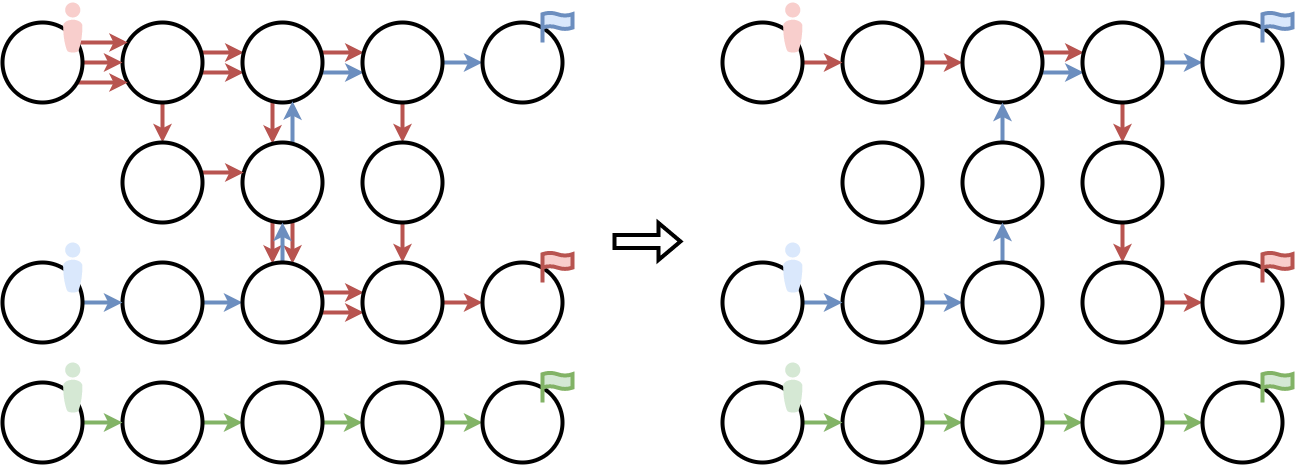
\includegraphics[width=9cm]{img/pm_example_intro.png}
\end{figure}

The approach in its definition is inspired and close to CBS's definition, however, the planning part of CBS stops if a conflict occurs and compute another time the planning part considering the conflict previously encountered, which is not the case for the Individual Path Finding; conflicts are handled after Individual Path Finding. 

Furthermore, our study shows that in certain cases, especially for large instances, our proposed approaches can outperform classical MAPF methods in terms of computation time. On the other hand, the results  outline the limits of the Plan Merging techniques we have developed. In certain scenarios, obtaining a complete solution might prove challenging or not feasible with the approaches we introduced, indicating the need to recognize the inherent limitations of the Plan Merging strategies.
\section{Background}\label{sec:background}

\subsection{MAPF}\label{sec:background_mapf}

The following definitions of Multi-Agent Path Finding (MAPF) follow the ones in~\cite{husvobbass22a}. MAPF is a triple $(V,E,A)$ where \(V,E\) denotes a connected graph, \(V\) being a set of vertices and \(E\) a set of edges connecting them, and \(A\) being a set of agents. For each agent \(a=(s,g) \in A\), \(s \in V\) denotes the starting location and \(g \in V\) denoting the goal location. Every starting position and every goal position are disjoint.
For each discrete time step \(t\in \mathbb{N}_0\), an agent can either, wait at its current vertex or move to a neighbouring one.

The output for MAPF problems is a plan \(\Pi\). A plan is a collection $(\pi_a)_{a\in A}$ of finite sequences in $(V,E)$ where each sequence $\pi_a$ is represented by a finite sequence of adjacent or identical vertices in $V$ from $s$ to $g$ for agent $a = (s,g)$. We use \(\pi_a (t) = v\) to denote that agent \(a\) is located at vertex \(v\) at time step \(t\). 
For each \(a=(s,g) \in A\), we have $\pi_a(0) = s$ and  $\pi_a(|\pi_a|-1) = g$, where $|\pi_a|$ gives the length of sequence $\pi_a$. Generally, for any \(a=(s,g)\) and any $0 \leq t \leq |\pi_a|-1$, we have \(\pi_a(t) \in V\). In addition, we also have $(\pi_a(t),\pi_a(t+1))\in E$ with $0 \leq t < |\pi_a|-1$

A plan is considered  \textit{valid} if, taken pair wisely, sequences are collision-free. A vertex conflict occurs whenever two different agents occupy the same vertex at the same time step. Formally, we have \(conflict(a,a',t)\) if given any $a,a'\in A$  and $t\in\mathbb{N}_0$, we have $\pi_a(t) = \pi_{a'}(t)$. An edge conflict (or swapping conflict) occurs whenever two agents exchange their position or are using the same vertex at the same time. We have \(conflict(a,a',t)\) if given any $a,a'\in in A$  and $t\in\mathbb{N}_0$, we have $\pi_a(t-1) = \pi_{a'}(t)$ and $\pi_a(t) = \pi_{a'}(t-1)$.

A plan $(\pi_a)_{a\in A}$ has a conflict, if a conflict $(a, a',t)$ occurs in $(\pi_a)_{a\in A}$ for some pair $a,a'\in A$ of agents and a time step $t\in\mathbb{N}_0$.

\textit{Sum-of-costs} and \textit{makespan} of a plan $(\pi_a)_{a\in A}$ are respectively defined as such; $\sum_{a\in A} (|\pi_a| - 1)$ and $\max_{a\in A} (|\pi_a| - 1)$.

Furthermore, we assume that graphs have Cartesian coordinate system, which means we can represent them as a grid. 

\subsection{ASP}

Answer Set Programming~\cite{ankolisc05a} (ASP)is an approach for declarative logic programming. In a nutshell, programmer aims to describe problems instead of solving them.

A logic program \(P\) is defined by a finite set of rules. Given a set of atoms \(\mathcal{A}\), a rule \(r\) is of the form 
\[
    a_0 \leftarrow a_1, \dots, a_n,not~a_{n+1}, \dots,not~a_m     
\] 
with \(a_i \in \mathcal{A}, 0 \leq i \leq m\). An atom preceded by \(not\) refer to its \textit{default negation}. We call literal an atom or its default negation.

In a rule \(r\), \(a_0\) represents the head of the rule and \(\{a_1, \dots, a_m,not~a_{m+1}, \dots,not~a_n\}\) the body of the rule. We will refer respectively to them as such; \(H(r)\) the head of the rule and \(B(r)\) the body of the rule. We define \(B(r) = B^+(r) \cup B^-(r) \) and \(B(P) = \{B(r) |r \in P\}\). For each rule \(r\) in \(P\), \(B^+(r) =\{ a_0 \leftarrow a_1, \dots, ~a_n\}\), \(B^-(r) =\{ a_{n+1}, \dots, ~a_m \}\) and \(H(r) = a_0\). 
A \textbf{fact} is defined as a rule with an empty body. On the other hand, with an empty head, the rule becomes an integrity \textbf{constraint}.
We define \(P_X\) as the reduct of a program \(P\) relative to a set of assigned atom \(X\).
\[
    P_X = \{H(r) \leftarrow B^+(r) | r \in P, X \cap B^-(r) = \emptyset\}
\]

A set \(X\) of atoms is a stable model of \(P\) if \(P_X\) is the smallest set under \(P_X\).



For instance, lets encode the following problem. We want to pack as many object in our bag respecting the maximum authorized weight. First lets denote the possible objects.

\begin{minipage}[H]{\linewidth}
\begin{lstlisting}[style=mystyle]
object(trousers, 3).
object(tshirt, 2).
object(toothbrush, 1).
object(camera, 2).
object(tent, 8).
object(drinks, 2).
object(sandwiches, 2).
object(laptop, 3).
object(tablet, 2).
\end{lstlisting}
\end{minipage}


To decide which objects to pick, we utilize a choice rule. A choice rule provide a choice over a set of atoms.

\begin{minipage}[H]{\linewidth}
\begin{lstlisting}[style=mystyle]
    {pick(N,W):object(N,W)}.
\end{lstlisting}
\end{minipage}

Here, the choice rule allows for various combinations of objects to be picked. We then enforce a constraint that ensures the total weight of the selected objects does not exceed 20. This constraint is expressed using an aggregate function within an integrity constraint:

\begin{minipage}[H]{\linewidth}
\begin{lstlisting}[style=mystyle]
    :- #sum{W : pick(N,W)} > 20. 
\end{lstlisting}
\end{minipage}

In addition, we add some normal rules and constraint to enforce \textit{picking} some items if some other items are picked. The first two constraint implies that, if the \textit{tent} object is picked, then it is not possible that \textit{drinks} and \textit{sandwiches} objects are not picked. The two last normal rules implies that, if \textit{laptop} and \textit{tablet} are picked, a \textit{charger} item is added to the pool of object and is picked.

\begin{minipage}[H]{\linewidth}
    \begin{lstlisting}[style=mystyle]
    :- pick(tent), not pick(drinks).
    :- pick(tent), not pick(sandwiches).
    
    object(charger,1) :- pick(laptop,W1), pick(tablet,W2).
    pick(charger,W) :- object(charger,W). 
\end{lstlisting}
\end{minipage}


Lastly, we want to maximize the weight of the bag while still keeping it under 20. To achieve this, we use an optimization statement that seeks to find the maximum weight among the available combinations:

\begin{minipage}[H]{\linewidth}
\begin{lstlisting}[style=mystyle]
    #maximize{W : pick(N,W)}. 
\end{lstlisting}
\end{minipage}
This encoding will yield the optimal combination of objects to pack into the bag, maximizing the weight without having the weight above 20.

\subsection{Solving MAPF with ASP}

\subsubsection{Instance Format}

A MAPF instance is defined using the following predicates

\begin{enumerate}
    \label{list:instance_format_explanation_part1}
    \item \(vertex/1\) which describe a vertex of the graph with a tuple \((X,Y), X,Y \in \mathbb{N}^+\) expressing the position.
    \item \(edge/2\) which describe an edge between two vertices. With two tuple \((X,Y), X,Y \in \mathbb{N}^+\) expressing the endpoints of the edge.
    \item \(agent/1\) which define agents of an instance with its identifier as parameter
    \item \(start/2\) which describe the starting position of an agent. With an agent identifier as first parameter and a vertex as second parameter expressing the starting position.
    \item \(goal/2\) which describe the goal position of an agent. With an agent identifier as first parameter and a vertex as second parameter expressing the goal position. 
\end{enumerate}

We introduce optional predicates used for the computation of individual paths. They are defined as such:

\begin{enumerate}
    \label{list:instance_format_explanation_part2}
    \item \(shortestpath\_length/2\)  represents the length of the shortest path of an agent. With the identifier of an agent as first parameter and the length of a shortest path for the associated agent.
    \item \(makespan/1\)  describes the maximum makespan of the instance. It can also be defined as a \(horizon\) constant
\end{enumerate}

For example, the following facts describe the graph illustrated by figure~\ref{lst:instance_format_example}.

\begin{minipage}[H]{\linewidth}
\begin{lstlisting}[style=mystyle, caption={Example of instance format}, label={lst:instance_format_example}]
agent(1). start(1,(2,1)). goal(1,(2,4)).
agent(2). start(2,(2,3)). goal(2,(2,5)).
agent(3). start(3,(5,4)). goal(3,(1,4)).

vertex((2,3)). vertex((1,4)). vertex((2,4)).
vertex((3,4)). vertex((4,4)). vertex((2,1)).
vertex((5,4)). vertex((2,5)). vertex((2,2)).

edge((2,4),(1,4)). edge((3,4),(2,4)).
edge((4,4),(3,4)). edge((5,4),(4,4)).
edge((2,3),(2,2)). edge((2,4),(2,3)).
edge((2,5),(2,4)). edge((2,2),(2,1)).
edge((2,3),(2,4)). edge((2,4),(2,5)).
edge((2,1),(2,2)). edge((2,2),(2,3)).
edge((1,4),(2,4)). edge((2,4),(3,4)).
edge((3,4),(4,4)). edge((4,4),(5,4)).

% Optional 
shortestpath_length(1,3).
shortestpath_length(2,2).
shortestpath_length(3,4).

makespan(4).
\end{lstlisting}
\end{minipage}


\begin{figure}[H]
    \centering
    \caption{Illustrated graph of the instance format example~\ref{lst:instance_format_example}}\label{fig:illustrated_instance_format_example}
    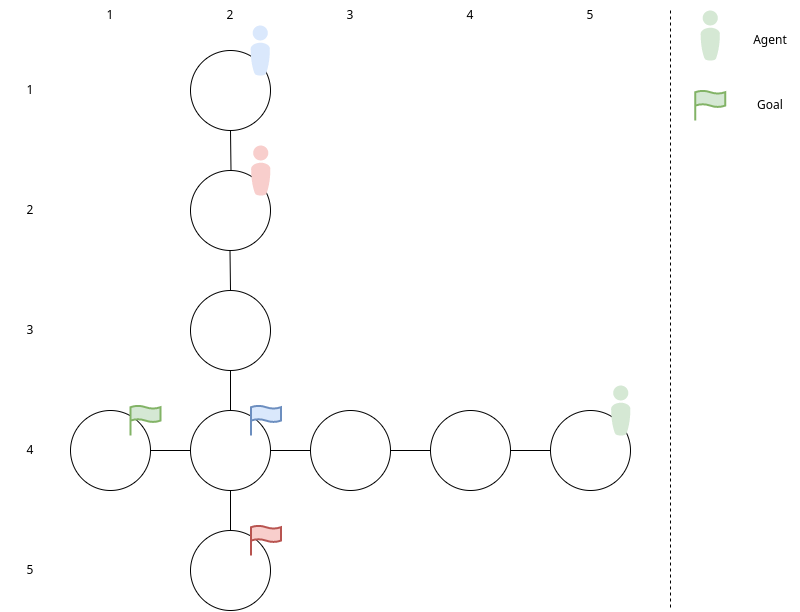
\includegraphics[width=\widthimg]{img/illustrated_instance_format_example.drawio.png}
\end{figure}


\subsubsection{Encoding}

As baseline for ASP MAPF solver, we adapt an encoding available in  \textit{asprilo}~\cite{geobotscsangso18a}, which we call \textbf{base MAPF encoding}. In the encoding, we use two primary predicates:

\begin{enumerate}\label{list:base_mapf_encoding_predicate_explanation}
    \item \(at(R,P,T)\)  represents the position \(P\) of an agent \(R\) at time step \(T\).
    \item \(move(R,U,V,T)\) represents the movement from vertex \(U\) to vertex \(V\) at time step \(T\).
\end{enumerate}

\begin{minipage}[H]{\linewidth}
\begin{lstlisting}[style=mystyle, caption={Base MAPF encoding}, label={lst:base_mapf_encoding}]
    at(R,P,0) :- start(R,P). |\label{line:init_at}|
    time(1..horizon). |\label{line:init_horizon}|

    {move(R,U,V,T) : edge(U,V)} 1 :- agent(R), time(T). |\label{line:generating_moves}|

    at(R,V,T) :- move(R,_,V,T). |\label{line:generating_at}|
    :- move(R,U,_,T), not at(R,U,T-1). |\label{line:constraining_moves}|
    at(R,V,T) :- |\label{line:waits}|
        at(R,V,T-1), 
        not move(R,V,_,T), 
        time(T). 

    :- { at(R,V,T) }!=1 , agent(R), time(T). |\label{line:one_at_per_t}|

    :- {at(R,V,T) : agent(R)} > 1, vertex(V), time(T). |\label{line:vertex_conflict}|
    :- move(_,U,V,T), move(_,V,U,T), U < V. |\label{line:edge_conflict}|
        
    :- goal(R,V), not at(R,V,horizon). |\label{line:goal_reached}|
\end{lstlisting}
\end{minipage}

In the initial section of encoding~\ref{lst:base_mapf_encoding}, we define, respectively on lines~\ref{line:init_at} and~\ref{line:init_horizon}, the starting positions of each agent and their allocated time using the constant \textit{horizon}.


The rule at line~\ref{line:generating_moves} describes how movements are performed. A possible interpretation could be; for each agent at each available time step and among all available edge going from \(U\) to \(V\), we pick at most one to define one movement at each time.

The rule at line~\ref{line:generating_at} states that if a move action is performed by the agent from any location (indicated by \textunderscore) to a different one, the agent is positioned at this destination at this time step.
Then, the rule at line \ref{line:constraining_moves} is a constraint that ensures consistency and coherence in the agent's locations over time. It prevents agents from moving towards a location without having been to the source location of the move at the previous time step. 
Furthermore, the rule at line~\ref{line:waits} specifies that if an agent does not make a move at a specific time step, their location remains the same. 
Rule \ref{line:one_at_per_t} ensures that an agent was at most one position at a time.

Line~\ref{line:vertex_conflict} outline vertex collision with a constraint rules;  for each vertex, at most one agent can be positioned at a vertex.
Secondly, the rule~\ref{line:edge_conflict} ensure that, no movement from vertex \(U\) to \(V\) and no movement from \(V\) to \(U\) are issued at the same time.
Lastly, the rules~\ref{line:goal_reached} forces that an agent is at their goal at the last timepoint.

The output of the encoding is the predicate \(at/3\). 

\section{Overview}

Plan merging involves the integration of multiple paths derived from various agents to construct a plan. Individual Path Finding~\ref{sec:ipf} which represent the computation part of multiple paths dor agents, can be a constituent of Plan Merging but it is not necessary.

The second step of Plan Merging is Path Selection~\ref{sec:pathselection}. Path Selection having the goal of identifying paths that closely resemble valid solutions to the problem at hand. However, it necessitates the construction of conflict-free set of path, which is computationally intensive, especially with a lot of agents and a lot of paths. This is where we incorporate Path Elimination to reduce the number of paths by eliminating potentially ``problematic'' paths using conflict-based strategy.

The final stage of Plan Merging involves obtaining a solution, which can be achieved by utilizing the pre-computed paths provided by Path Selection, by using the paths in their original form, or by employing the delineation of the pre-computed paths as a subgraph in order to reduce complexity for a MAPF algorithm.


The following figure~\ref{fig:overview} shows the different part of Plan Merging, having in order, Individual Pathfinding, Path Selection and Solving.

\begin{figure}[H]
    \centering
    \caption{Overview of the thesis}\label{fig:overview}
    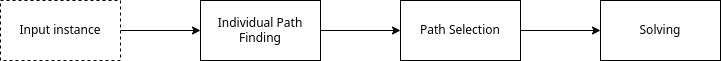
\includegraphics[width=\widthimg]{img/overview.drawio.png}
\end{figure}



\chapter{Individual Path Finding}
\label{sec:ipf}
This chapter describes how Individual Path Finding is formalized and how computation can be achieved using ASP and Clingo. 

\begin{figure}[H]
    \centering
    \caption{Overview of IPF}\label{fig:overview_ipf}
    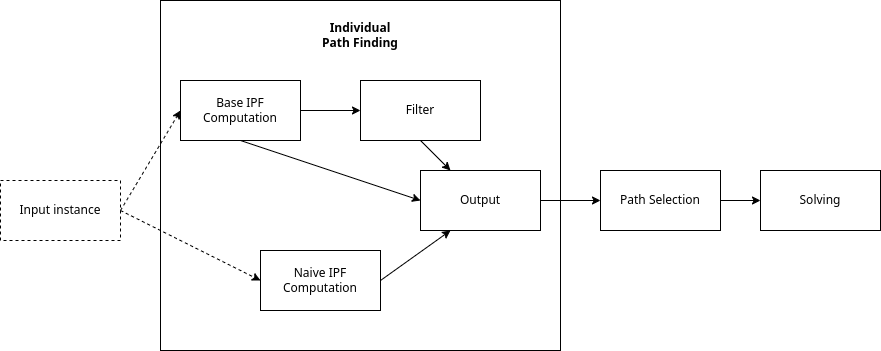
\includegraphics[width=\widthimg]{img/overview_ipf.drawio.png}
\end{figure}

\section{Formalization}

Individual Path Finding~\cite{luis2020plan,delling2009engineering} (IPF) represents the computation of multiple paths for each agent without considering collision in a given MAPF problem. The idea is then to use the paths for Plan Merging. We formalize IPF as a triple \((V,E,A)\) which is defined as in MAPF. The output is a non-empty set of set of paths \(\tau\). For each agent \(a \in A\), we have \(\tau[a]\) = \(\{\pi_0,\dots,\pi_n\}\). For lighter notation, we write \(\gamma_a = \tau[a]\), and also \(\gamma\) to refer to a set of path in general. Paths composing \(\gamma\) can be of different length. The following figure illustrate a \(\tau = \{\gamma_r, \gamma_b, \gamma_g\}\) where \(|\gamma_r|=3\), \(|\gamma_b|=1\) and  \(|\gamma_g|=1\). 

\begin{figure}[H]
    \centering
    \caption{Example of a \(\tau = \{\gamma_r, \gamma_b, \gamma_g\}\)}\label{fig:ipf_example}
    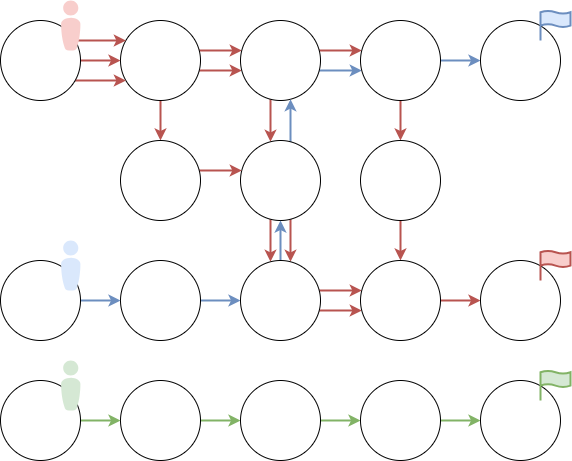
\includegraphics[width=\widthimg]{img/ipf_example.drawio.png}
\end{figure}


Paths can have different inner properties such as, length, number of bends, coverage of the graph or inter-connected properties such as number of plan conflict, diversity, distance and so on. The work achieved in the thesis has been made considering only length of paths, potential conflict, diversity and distance.

Path length is a very important property. We can splits paths into two length category; shortest paths, and non-shortest path.

\subsection{Diversity and Distance}

Diversity evaluates the variety of used vertices for a given set of paths of an agent. We introduce diversity as a sum of unique vertices visited at each time step. The function described in~\ref{math:diversity_formula} computes diversity for a given \(\gamma\).The formula is based on the Hamming distance~\cite{hanaka2022computing}. 

\begin{equ}[H]
    \begin{equation}\label{math:diversity_formula}
        distance(\gamma) = |\bigcup^{\pi \in \gamma}{(\cup^{v,t \in \pi}{(v,t)})}|
    \end{equation}
    \caption{Diversity function definition}
\end{equ}

Other diversity computation can be used, such as the Jaccard coefficient~\cite{habochal21a}. The difference between Jaccard coefficient and Hamming distance is that the first one focuses on the number of nodes that two paths have in common, while the second one focuses on the number of differences between the two paths. For our purpose, Hamming distance is more appropriate, however, it require that set are of the same length. Since paths in \(\gamma\) can be of different length, an adapted function was necessary. Note that the function~\ref{math:diversity_formula} do not gives an index that can be compared to other \(\gamma\)'s diversity. Furthermore, this equation is easy to implement with Clingo.

On the other hand, we can compute distance among paths in a \(\gamma\). Taken pair wisely, the distance between two paths is the sum of the distance between the vertices at each time step. Note that the distance between two vertices each be an arbitrary function such as euclidean distance or the shortest path length between these two vertices. We refer to this arbitrary function as \(dist(v,v')\). In our case, we consider \(dist(v,v')\) as the euclidean distance between \(v\) and \(v'\). The formalization of the distance for a given \(\gamma\) is defined in the following equation~\ref{math:distance_formula}. 

\begin{equ}[H]
    \begin{equation}\label{math:distance_formula}
        diversity(\gamma) = \mathlarger{\sum_{\pi,\pi' \in \gamma, \pi \neq \pi' }}{(\sum_{t=0}^{t \rightarrow min(|\pi|,|\pi'|)}{dist(\pi[t],\pi'[t])})}
    \end{equation}
    \caption{Diversity function definition}
\end{equ}


Figure~\ref{fig:diversity_vs_distance} shows two \(\gamma\) of size \(|\gamma|=2\). The first one shows an example of the most diverse \(\gamma\) possible for this problem (multiple solutions exist, and we consider paths in \(\gamma\) of same length). On the other side, we have an example of the most distant \(\gamma\) possible for this problem. Red squares illustrate the difference between diversity and distance.

\begin{figure}[H]
    \centering
    \caption{Diversity vs Distance}\label{fig:diversity_vs_distance}
    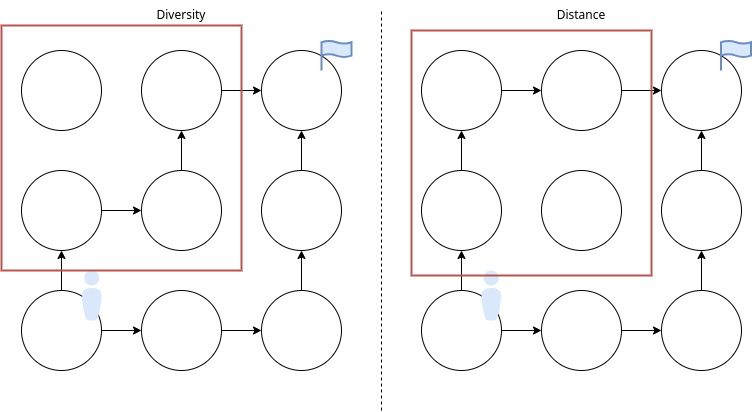
\includegraphics[width=\widthimg]{img/diversity_vs_distance.drawio.png}
\end{figure}



\section{Computation}


In this subsection, we present two different approaches for computing multiple paths. Even though IPF constitutes a side topic for this thesis, a concern was to be able to compute \(x\) paths for each agent within a reasonable time. We implemented the following computation approaches using Clingo (ASP). Computing paths with programming languages such as C, C++, Rust, and so on might offer better speed. We opted to stick with Clingo for its straightforwardness and technology consistency throughout this work. This section may serve as a starting point for future work on computing multiple paths using ASP and Clingo.

\subsection{Naive IPF Computation}\label{sec:naive_ipf_computation}

The first approach that we describe is a direct modification of the encoding presented in the section~\ref{sec:introduction}. The copy adds a new constant to the encoding called \textit{npaths} which denotes the number of paths to compute per agent. We modify \(at/3\) and \(move/4\) predicates, by adding a new argument being the identifier of the path. A unique path is now defined with an agent \(R\) and a path identifier \(I\). With these new directives, we obtain an encoding that we  call \textbf{Naive IPF}~\ref{lst:naive_ipf} which computes multiple paths for each agent in one call.

\begin{minipage}[H]{\linewidth}
\begin{lstlisting}[style=mystyle, caption={Naive IPF computation}, label={lst:naive_ipf}, numbers=left, ,escapechar=|]
    agent(R,1..npaths) :- agent(R). |\label{line:agent_id_and_path_id}|
    
    at(R,I,P,0) :- start(R,P), agent(R,I).

    time(1..horizon).
    {move(R,I,U,V,T) : edge(U,V)} 1 :- agent(R,I), time(T). |\label{line:move4_to_move5}|

    at(R,I,V,T) :- move(R,I,_,V,T). |\label{line:at3_to_at4}|
    :- move(R,I,U,_,T), not at(R,I,U,T-1).

    at(R,I,V,T) :- 
        at(R,I,V,T-1), 
        not move(R,I,V,_,T),
        time(T).

    :- { at(R,I,V,T) }!=1 , agent(R,I), time(T). 

    :- goal(R,V), not at(R,I,V,horizon).
\end{lstlisting}
\end{minipage}

The encoding in Listing~\ref{lst:naive_ipf} has the exact same principles as the base MAPF encoding (see Listing~\ref{lst:base_mapf_encoding}). Line~\ref{line:agent_id_and_path_id} introduces id \(I\) for paths. Note that in this case, all agents would have the same number of paths. We could use other predicates to describe how many paths are required for each agent of an instance. Lines~\ref{line:move4_to_move5} and~\ref{line:at3_to_at4} shows predicates \textit{move/4} and \textit{at/3} getting changed to predicates \textit{move/5} and \textit{at/4} now including the ID of paths.


The main flaw that comes with the encoding described is slowness. Requesting multiple paths per agent raises the search-space considerably. Even if we remove conflict consideration in the encoding,  the grounder needs to ground the rules containing predicate \(move/5\) at most \(|A| * npaths\) time. In addition, more variables induce a slower solving. 
However, this encoding gives us the opportunity to add properties to paths. For example, to implement diversity\ref{math:diversity_formula}, we can use an optimization statement:

\begin{minipage}[H]{\linewidth}
\begin{lstlisting}[style=mystyle]
    #maximize{1,R,V,T : at(R,I,V,T)}.
\end{lstlisting}
\end{minipage}

More definitive additions such as constraining specific paths of specific agents to have a defined length, a defined number of bends and so on, could be used.
Another flaw that comes with this encoding is that there is no guarantee that all paths for the same agent are different. However our \textbf{Naive IPF} encoding would still compute the requested number of paths for this agent \(a\) even though paths are the same. This can be fixed using collision for individual agents; the risk could be to revert to classical MAPF solving.

\subsection{Base IPF computation}\label{sec:base_ipf_computation}

By using multi-shot solving and assumptions~\cite{karoscwa21a}, it is  possible to ground both predicates \(at\) and \(move\) once for all agents. To do so, we tweak the naive IPF encoding described in section~\ref{sec:naive_ipf_computation} and obtain the encoding in Listing~\ref{lst:base_ipf}. This encoding can be interpreted as simple pathfinding that will be executed one agent at a time. Furthermore, \(start/2\) and \(goal/2\) predicates are not necessary; these are handled by assumptions.


\begin{minipage}[H]{\linewidth}
\begin{lstlisting}[style=mystyle, caption={Base IPF computation}, label={lst:base_ipf}]
    time(1..horizon).

    {at(V,0) : vertex(V)} = 1.

    { move(U,V,T) : edge(U,V)} 1 :- time(T).

    at(V,T) :- move(_,V,T).
    :- move(U,_,T), not at(U,T-1).

    :- { at(V,T) } != 1, time(T).

    at(V,T) :- at(V,T-1), not move(V,_,T), time(T).

    current_agent(R) :- at(V,0), start(R,V). |\label{line:identify_current_agent}|
    at(GV,T) :- at(GV,T-1), time(T), goal(R,GV), |\label{line:stay_after_goal_reached}| 
             current_agent(R). 
\end{lstlisting}
\end{minipage}

Line~\ref{line:identify_current_agent} aims to identify the current agent the solver is generating paths for. Through the assumption of the predicate \(at/2\) at time step 0, we can retrieve the current agent using the corresponding \(start/2\) predicate. Line~\ref{line:stay_after_goal_reached} is then designed to guarantee that once the path of an agent reaches its goal, the agent remains at its goal location.


The flowchart described in figure~\ref{fig:flowchart_ipf_computation} illustrates the process of base IPF computation. It first ground the instance with the encoding, then solve with the start and goal positions of an agent as assumptions. Finally, it extends \textit{at/2} with agent ID and model number. We use the model number to identify different paths of the same agent; the model enumeration represents different possible assignations for the problem. Requesting \(n\) models means requesting \(n\) paths for an agent.

\begin{figure}[H]
    \centering
    \caption{Flowchart of IPF computation using multi-shot solving and assumption}\label{fig:flowchart_ipf_computation}
    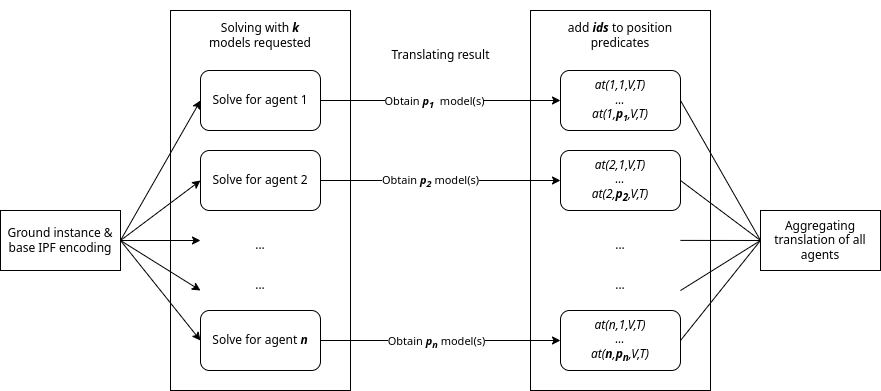
\includegraphics[width=\widthimg]{img/flowchart_ipf_computation.drawio.png}
\end{figure}


We define \(1 \leq p \leq k\), if solving an instance with \(k\) requested models, the number of possible models \(p\) can be lower. 
We use a Python wrapping to control and manage assumptions. A pseudocode of the wrapper is denoted in Listing~\ref{lst:pseudo_code_ipf_wrapper}

\begin{minipage}[H]{\linewidth}
\begin{lstlisting}[style=mystyle, caption={Pseudo code of base IPF encoding wrapper}, label={lst:pseudo_code_ipf_wrapper}, numbers=left, ,escapechar=|]
    result |\(\leftarrow\)| list()
    ground(instance + base IPF encoding)

    for each agent in instance |\{|
        assume(initial and goal position)
        solve()

        for each model |\{|
            translate `at/2'|\(\rightarrow\)|`at/4'
            add translation to result
        |\}|
    |\}|  
\end{lstlisting}
\end{minipage}

A nice property that comes with this approach is that since we use model enumeration to create different paths, if Clingo enumerates fewer models than requested, we can assume that there are no other paths possible of this length.

Base IPF computing reduces computation time significantly; given the way Clingo works, decomposing the problem into one agent at a time and reusing grounding works is faster than trying to solve multiple problems at once. It does, however, compute random paths. In order to compute the shortest paths, we can use the optional predicates described in list~\ref{list:instance_format_explanation_part2}. Assumptions allow us to force \(goal/2\) predicate to be reached a specific time step,  We can then change the goal position assumption and force it to be reached at a certain time step instead of at the horizon. We can use the same principle to compute paths of different lengths for one agent; this requires an additional solving and translation step.

Furthermore, in this process, we can compute additional paths with a modified time step associated with the goal. This addition enables agents to reach their destination xx time steps later than the originally defined duration. This strategy proves valuable when a limited number of paths are computed, as it provides the IPF solver with extra possibilities to generate additional paths.

Given the way base IPF computation works, it seems difficult to assign different properties to the paths that depends on other paths. Properties, such as, length, number of bends can easily be achieve. On the other hand, diversity and distance seems difficult. To achieve a similar result, we can request a large number of paths and create a subset out of them that satisfy chosen properties. 






\subsection{Filters}

Compared to naive IPF computation, properties depending on other paths seem difficult to compute. We can however create subset of previously computed \(\gamma\) by filtering paths given some criteria. A filter \(f\) is defined as such; \( f(\gamma) \subseteq \gamma \). We introduce two criteria functions. The first being a function selecting \(k\) most diverse paths following~\ref{math:diversity_formula} and the second one a function selecting \(k\) most distant paths following~\ref{math:distance_formula}.

\begin{minipage}[H]{\linewidth}
\begin{lstlisting}[style=mystyle, caption={Encoding of diverse filter}, label={lst:diversity_filter}, numbers=left, ,escapechar=|]
    #const npath = 5.

    {dpath(R,I): at(R,I,_,_)} npath :-  agent(R). |\label{line:div_select_path_p1}|
    #maximize {1@2,R,I : dpath(R,I)}. |\label{line:div_select_path_p2}|
    
    dpath(R,I,V,T) :- dpath(R,I), at(R,I,V,T). |\label{line:div_retrieving_pos}|
        
    #maximize {1@1R,V,T : dpath(_,_,V,T)}. |\label{line:maximizing_diversity}|
\end{lstlisting}
\end{minipage}

The diversity encoding in Listing~\ref{lst:diversity_filter} starts by picking, for each agent, at most \textit{npath} paths among all path available denoted in line~\ref{line:div_select_path_p1}. Line~\ref{line:div_select_path_p2} maximize the amount of chosen paths. Using this optimization statement, we avoid unsat results when not enough paths exist for an agent. Line~\ref{line:div_retrieving_pos} retrieves positions and time steps of selected paths. From these selected path, we can count the tuple \((V,T)\) and maximize them with the optimization statement in line~\ref{line:maximizing_diversity}.

\begin{minipage}[H]{\linewidth}
\begin{lstlisting}[style=mystyle, caption={Encoding of distance filter}, label={lst:distance_filter}, numbers=left, ,escapechar=|]
    #const npath = 5.

    {dpath(R,I): at(R,I,_,_)} npath :-  agent(R). |\label{line:dist_select_path_p1}|
    #maximize {1@1,R,I : dpath(R,I)}. |\label{line:dist_select_path_p2}|
    
    dpath(R,I,V,T) :- dpath(R,I), at(R,I,V,T).|\label{line:dist_retrieving_pos}|
         
    dist(R,I1,I2,T, (X1-X2)*(X1-X2) + (Y1-Y2)*(Y1-Y2)) :- |\label{line:dist_computing_distance}|
        dpath(R,I1,(X1,Y1),T),  
        dpath(R,I2,(X2,Y2),T), I1!=I2. 

    dsum(R,DS) :- |\label{line:dist_intermediate}|
        DS=#sum{D:dist(R,I1,I2,_,D), dpath(R,I1), dpath(R,I2)}, 
        agent(R).

    #maximize {1@2,D : dsum(R,D)}.|\label{line:maximize_distance}|
\end{lstlisting}

\end{minipage}


The distance encoding Listing~\ref{lst:distance_filter} starts by picking for each agent, at most \textit{npath} paths among all path available, maximizing the number of selected path and then retrieving their position and time step (from line~\ref{line:dist_select_path_p1} to~\ref{line:dist_retrieving_pos}). Line~\ref{line:dist_computing_distance} introduces a new predicate \(dist/4\) which denotes  euclidean distance of two different paths of the same agent. We then have an intermediate rule line \ref{line:dist_intermediate} which sums the distance of paths for each agents. It is then used in the optimization statement in line~\ref{line:maximize_distance} to maximize the distance issued by \(D\).

\chapter{Path Selection}
\label{sec:pathselection}

In this chapter, we will describe what Path Selection (PS) is, how it works and which strategies we use to take advantage of multiple computed paths per agent. Figure~\ref{fig:overview_merging} shows the different steps for Path Selection used in this work.

\begin{figure}[H]
    \centering
    \caption{Overview of Path Selection}\label{fig:overview_merging}
    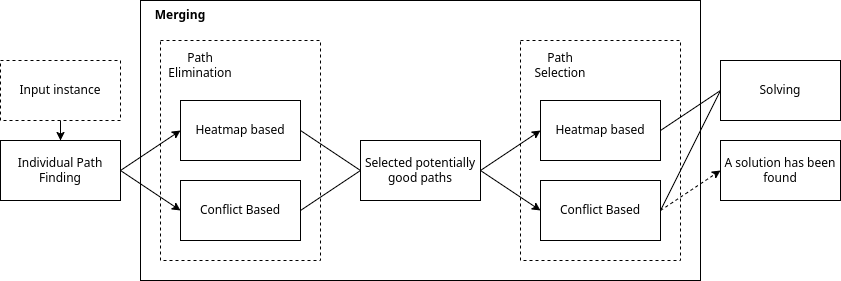
\includegraphics[width=\widthimg]{img/overview_merging.drawio.png}
\end{figure}


Path Selection takes a \(\tau\) as its input and produces a subcomponent \(\tau'\) when \(\forall a \in A \text{ } | \text{ } \gamma'_a \in \tau' \subseteq \gamma_a \in \tau\). Furthermore \(\tau'\)  denotes a plan, where \(\forall \gamma'_{a \in A' \subseteq A}\in \tau',| \gamma'_a|=1 \). 


\section{Heatmap}

Heatmap is about projecting likelihood of presence of an agents on vertices at each step. Inspired from papers~\cite{atstfestko20a, banatu02a}. Likelihood refers to, in a scope of an agent, the probability of be being at a specific vertex for each time step according to a set of path \(\gamma\). This heatmap interpretation stands for the scope of one agent. We will refer to single agent heatmap as \textbf{Individual Heatmap} (IH). We formalize, in equation~\ref{math:individual_heatmap} an Individual Heatmap function:

\begin{equ}[H]
    \begin{equation}\label{math:individual_heatmap}
        \phi(\gamma,v,t) = \frac{| \{\pi|\pi \in \gamma,\pi(t) = v\}|}{|\gamma|}
    \end{equation}
    \caption{Individual Heatmap}
\end{equ}


\(\phi\) is calculated --  given a \(\gamma\) of an agent, a vertex and a timepoint. For example, we can compute the Individual Heatmap of a given \(|\gamma|=3\) illustrated in figure~\ref{fig:individual_heatmap}.

\begin{figure}[H]
    \centering
    \caption{Example of Individual Heatmap computed from a \(|\gamma|=3\)}\label{fig:individual_heatmap}
    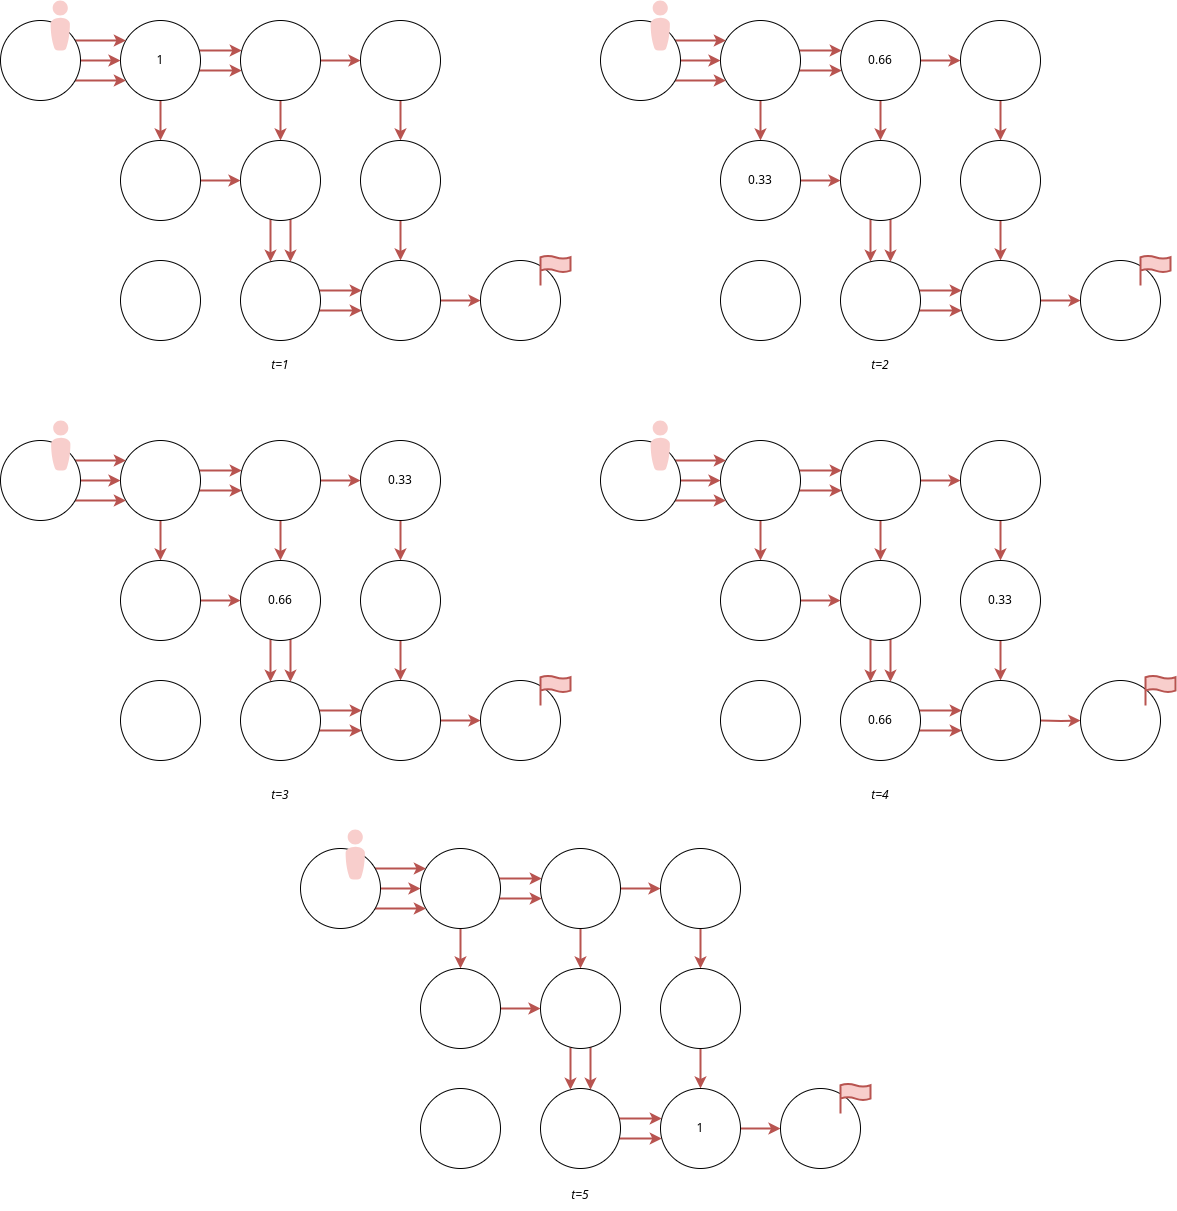
\includegraphics[width=\widthimg]{img/individual_heatmap.drawio.png}
\end{figure}

This representation produces critical vertices for an agent, where higher values correspond to a greater likelihood of vertex utilization. On the other hand, the mean heatmap value associated with \(\gamma\) serves as an indicator of path diversity, with elevated values signifying a low level of path diversity.

We derive a \textbf{Global Heatmap} (GH) through the aggregation of all Individual Heatmaps. It is important to note that Global Heatmaps, in this context, no longer serve as a direct indicator of the likelihood of presence but instead an indicator of ``usage of vertices'' .

A Global Heatmap \(\Phi\) of \(\tau\) is formalized in the following equation~\ref{math:global_heatmap}. As for Individual Heatmaps, a Global Heatmap value of \(\Phi\) is computed given a vertex \(v\) and a time step \(t\).  

\begin{equ}[H]
    \begin{equation}\label{math:global_heatmap}
        \Phi(\tau,v,t) = \frac{ \sum_{\gamma \in \tau}\phi(\gamma,v,t)}{|\tau|}
    \end{equation}
    \caption{Global Heatmap}
\end{equ}


To perform the computation of Individual Heatmaps and Global Heatmaps using Clingo, it is important to consider that Clingo inherently rounds down floating-point numbers. To obtain accurate heatmaps values in our context, we require an external program capable of performing divisions without rounding down the result.
We introduce the encoding of the Individual Heatmap in listing\ref{lst:individual_heatmap_encoding}.

\begin{minipage}[H]{\linewidth}
\begin{lstlisting}[style=mystyle, caption={Individual Heatmap encoding}, label={lst:individual_heatmap_encoding}]
    individual_heatmap(R,V,T,(K,N)) :- 
        K = #count{1,I : at(R,I,V,T)}, |\label{line:ihm_counting_paths}|
        N = #count{1,I : at(R,I,_,_)}, |\label{line:ihm_counting_all_paths}|
        at(R,_,V,T).  
\end{lstlisting}
\end{minipage}


This short encoding introduces  \(heatmap/4\) predicates, with \(R\), \(V\) and \(T\) being respectively the agent ID, a vertex and a time point. The last argument of the predicate is a tuple \((K,N)\) where \(K\), computed on line~\ref{line:ihm_counting_all_paths}, is the number of paths of \(R\) that go through \(V\) at time step \(T\). And \(N\), computed on line~\ref{line:ihm_counting_all_paths}, denotes the number of paths that belong to the agent \(K\).

The calculation of the Global Heatmap is performed using \textbf{Python}\footnote{It is possible to provide the nominator and the denominator for the Global Heatmap at each vertex and each time step, however, compared to using a third-party programming language, it is very slow or not computationally feasible in practice.}.


\section{Path Elimination}

Path Elimination (PE) is the process of the removing paths that exhibit potential issues. It serves to chunk through the multitude of possible paths and eliminate those that are deemed ``potentially problematic''. This step serves as a preprocessing stage for Path Selection (PS). 

Figure~\ref{fig:overview_merging_path_elemination} sums up the different processes in order to eliminate potentially-conflicting-paths.

\begin{figure}[H]
    \centering
    \caption{Overview of Merging: Path Elimination}\label{fig:overview_merging_path_elemination}
    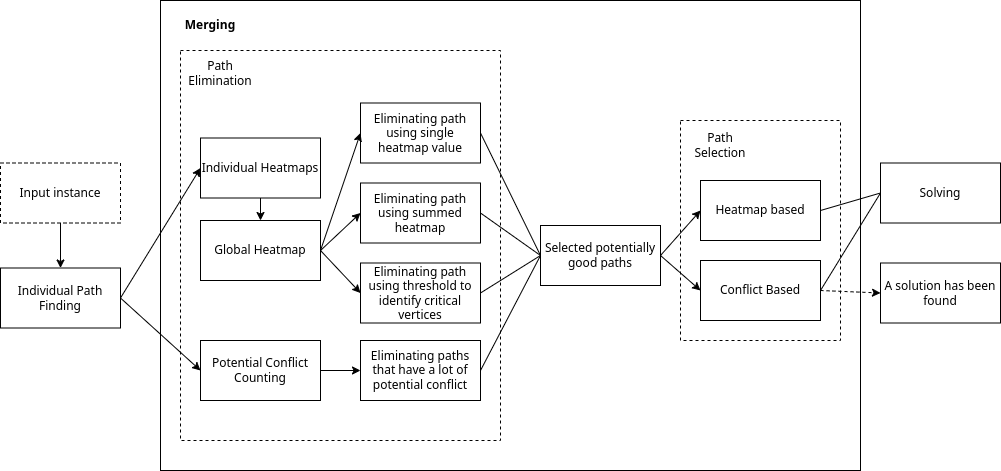
\includegraphics[width=\widthimg]{img/overview_merging_path_elimination.drawio.png}
\end{figure}

We first introduce some definition.

\begin{definition}
    A path is classified as \textbf{killed} when it has been explicitly removed of the output of Path Elimination.
\end{definition}

\begin{definition}
    A path is classified as \textbf{selected} when it has been explicitly selected for the output of Path Elimination.
\end{definition}

\begin{definition}
    An agent is classified as \textbf{killed} when all of its paths have been explicitly killed during the Path Elimination process.
\end{definition}

\begin{definition}
    A vertex can be classified as \textbf{critical} at a certain time step by a Path Elimination process. It assume that there is high chance of collision.
\end{definition}

\begin{definition}
    An agent is classified as \textbf{critical} when at least one of the vertices composing its plan is considered as \textbf{critical} in each of its paths.
\end{definition}

\begin{definition}
    A \textbf{potential conflict} denotes conflict among paths of different \(\gamma\). It do not represent an actual conflict.
\end{definition}



\subsection{Using Global Heatmap}

Global Heatmap values often provide insights into vertices that are prone to conflicts. This information can be leveraged for path elimination. 

A simplistic approach involves minimizing the cumulative Global Heatmap value by allowing the encoding select or not paths for the computation of GH. Unfortunately, due to the interconnections among heatmaps, practical grounding of this approach becomes feasible only on small instances.

We then present three approaches for identifying potentially conflicting paths in a reasonable computation time.

\subsubsection{Eliminating paths using unique heatmap value}

One straightforward approach involves ordering all possible assignments of \((v, t)\) within a given \(\tau\) based on their global heatmap values. We classify the top \(k\) vertices as ``critical''. Which can then be used as reference points for path elimination based on various criteria. We can identify which paths pass through critical vertices using the following rule:

\begin{minipage}[H]{\linewidth}
\begin{lstlisting}[style=mystyle]
    critical_path(R,I,V,T) :- 
        critical_vertex(V,T), 
        at(R,I,V,T), 
        not path_killed(R,I).
\end{lstlisting}
\end{minipage}


We then determine \(n\) critical paths that should be eliminated. For instance, we may opt to eliminate half of them as follows:

\begin{minipage}[H]{\linewidth}
\begin{lstlisting}[style=mystyle]
    {to_kill(R,I): critical_path(R,I,V,T) } = K/2 :-
        K = #count{1,R',I' critical_path(R',I',V,T)},
        critical_vertex(V,T).
\end{lstlisting}
\end{minipage}

Note that we use predicate\(to\_kill/2\) and \(path\_killed/2\) that refer to the same concept. We do differentiate them so the paths that are yet to be eliminated (\(to\_kill/2\)) do not interfere with already killed paths (\(path\_killed/2\)).  

There are various parameters and variations to consider in determining the value that \(n\) can take. These may include individual heatmap values, whether an agent has already had some of its paths eliminated

The approach we settle on is the following;

\begin{figure}[H]
    \centering
    \caption{Eliminating paths using unique heatmap value}\label{fig:simple_heatmap_value_elimination}
    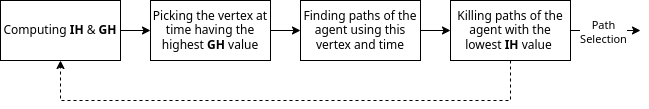
\includegraphics[width=\widthimg]{img/simple_heatmap_value.drawio.png}
\end{figure}

As illustrated in figure~\ref{fig:simple_heatmap_value_elimination}, it is possible to loop the process to eliminate more paths. 

As mentioned earlier, the lack of floating-point number handling of Clingo forces us to use a Python wrapper to sort Global and Individual Heatmap values.

The decision to eliminate paths of agents with the lowest Individual Heatmap values can be justified on two grounds:
\begin{enumerate}
    \item \textbf{Node Importance}: Higher Individual Heatmap values signify that a particular vertex holds more significance at this time step for the respective agent. Consequently, it is more suitable to eliminate paths of agents with lower interest in this vertex, as they are less likely to utilize it.
    \item \textbf{Balanced Elimination}: Opting to eliminate paths of agents with low Individual Heatmap values helps maintain a balanced elimination process; selecting agent with the lowest heatmap means killing the least possible paths involved in the \textbf{critical vertex}. It allows us to not kill agents too swiftly. 
\end{enumerate}

If we apply the previous approach explained above, on the example illustrated on figure ~\ref{fig:ipf_example}. We highlighted global heatmap in red at the critical moment (time step \(t=3\)), see figure~\ref{fig:simple_heatmap_value_elimination_example}. 

\begin{figure}[H]
    \centering
    \caption{Eliminating paths using unique Global Heatmap value process example}\label{fig:simple_heatmap_value_elimination_example}
    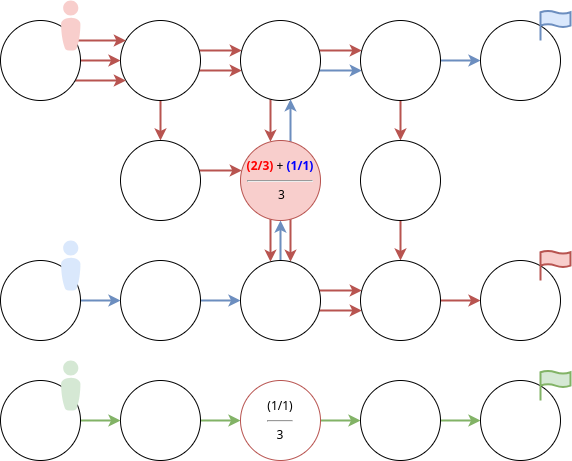
\includegraphics[width=\widthimg]{img/pe_one_heatmap_value_example.drawio.png}
\end{figure}

Between the two highlighted vertices, according to the elimination process~\ref{fig:simple_heatmap_value_elimination}, the vertex with the highest Global Heatmap value is the one colored in red. From this vertex, we can denote three paths going through it at time step \(t=3\). We then order the Individual Heatmap values of the two concerned agents, blue and red. from these values we can deduce that the two paths of red agents have to be killed. We obtain figure~\ref{fig:simple_heatmap_value_elimination_example} which is in this case a valid plan:

\begin{figure}[H]
    \centering
    \caption{Result of eliminating paths using unique heatmap value process}\label{fig:simple_heatmap_value_elimination_example_result}
    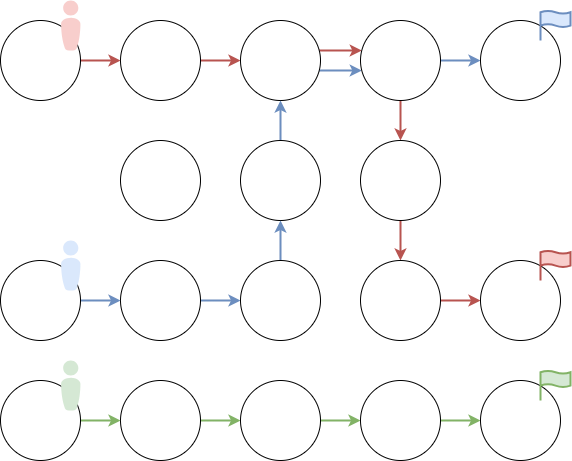
\includegraphics[width=\widthimg]{img/pe_one_heatmap_value_example_result.drawio.png}
\end{figure}

Nevertheless, despite our efforts to implement strategies aimed at balancing the elimination process among agents, adopting a vertex-oriented approach tends to kill agents swiftly.

\subsubsection{Eliminating paths using GH threshold}

One flaw that comes with the previous approach is that the process is doing one vertex after an other. It is difficult to define a value that eliminate the right amount of paths to be relevant. We propose a way to identify multiple critical vertices in one call.

The principle is simple, if the Global Heatmap value of a vertex at a specific time point is higher than a defined value \(\mathcal{H}\), the vertex is denoted as critical. We call this defined value a \textbf{threshold}. Formally, we have;

\begin{equ}[H]
    \begin{equation}\label{math:critical_vertex_threshold}
        critical\_vertices(\tau) = \{(v,t) | \Phi(\tau,v,t) > \mathcal{H}(v,t) \in \mathcal{F}(\tau) \} 
    \end{equation}
    \caption{Identifying critical vertices using threshold}
\end{equ}

Where \(\mathcal{F}\) is a function enumerating all possible tuple \(v,t\) in \(\tau\):

\[
    \mathcal{F}(\tau) = \mathlarger{\mathlarger{\bigcup_{\gamma\in\tau}}}\bigcup_{\pi\in\gamma}\cup_{t=0}^{t \rightarrow |\pi|}{(\pi[t],t)}
\]


Threshold values can be defined through different equations, considering different properties. Equation~\ref{math:simple_biased_threshold}, denoted as \(\mathcal{H}_{sbt}(A,\Delta)\), defines a simple biased threshold. In essence, without considering the bias, this equation implies that a vertex is labeled critical if, for all \(n\) agents with \(k\) paths each, \(\frac{1}{n}\) of their paths utilize this vertex at a specific time plus one additional path. The bias adjustment allows for the flexible inclusion of more or less critical vertices.

\begin{equ}[H]
    \begin{equation}\label{math:simple_biased_threshold}
        \mathcal{H}_{sbt}(A,\Delta) =  \frac{1*\Delta}{|A|}
    \end{equation}
    \caption{Simple (biased) threshold}
\end{equ}



The simplicity of the basic threshold equation makes it a general tool, but it lacks vertex-specific context. To address this limitation, we introduce a more sophisticated approach with a context-dependent threshold in equation~\ref{math:contextdependant}. This threshold calculation takes into account the number of paths using a particular vertex at a specific time step (\(T\)) and the number of agents involved, providing a more precise evaluation of critical vertices. The equation incorporates a bias factor \(\Delta\) that is used for finetuning.

\begin{equ}[H]
    \begin{equation}\label{math:contextdependant}
        \mathcal{H}_{bcdt}(V,T,A,\Delta) = \frac{npath\_on(V,T)*\Delta}{nagent\_on(V,T) * |A|}
    \end{equation}
    \caption{(Biased) Context dependent threshold}
\end{equ}


\subsubsection{Eliminating paths using sums of heatmap values}

In contrast to a vertex-oriented approach, which may label a path as "critical" even if it possesses critical attributes only on a single occurrence. An alternative strategy involves considering the scope of entire paths that may highlight conflict. The approach entails assigning a value to an entire path by summing the Global Heatmap values associated with its vertices. The approach is outlined in figure~\ref{fig:summed_heatmap_value_elimination}. 

\begin{figure}[H]
    \centering
    \caption{Eliminating paths using summed Global Heatmap values process overview}\label{fig:summed_heatmap_value_elimination}
    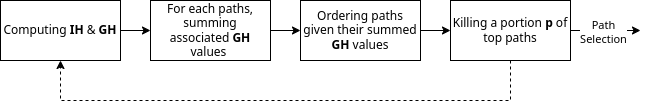
\includegraphics[width=\widthimg]{img/summed_heatmap_value.drawio.png}
\end{figure}

This approach tends to kill agents quite quickly when only a few paths are involved. However, it tends to be more efficient the more diverse \(\gamma\in\tau\) are. Futhermore, with one call, this approach can chunk a significant portion of the paths. 


\subsection{Using conflicts}

We introduce a fourth approach that centers around \textbf{potential conflicts} to guide Path Elimination. In this method, for each agent and at every vertex along their path, we calculate the count of \textbf{potential conflicts}. This approach stands apart from the heatmap-based methods in a significant way: when an agent possesses a substantial number of paths, their individual paths do not significantly influence the Global Heatmap values, even if they have the potential to cause conflicts. However, in the Potential Conflict-based approach, every path is treated with equal weight.

The encoding for the described approach is defined in Listing~\ref{lst:conflict_based_path_elimination}.


\begin{minipage}[H]{\linewidth}
\begin{lstlisting}[style=mystyle, caption={Conflict-based Path Elimination}, label={lst:conflict_based_path_elimination}]
    #const n = 5.

    to_determine(R,I) :- at(R,I,_,_), not path_killed(R,I). |\label{line:to_determine}|

    potential_conflict(R,I,V,T) :- |\label{line:potential_conflict}|
        to_determine(R,I), at(R,I,V,T), 
        to_determine(R',I'), at(R',I',V,T), 
        R'!=R.

    path_composition(R,I,C) :- |\label{line:path_composition}|
        C = #count{1,V,T : potential_conflict(R,I,V,T)}, 
        to_determine(R,I).

    {to_kill(R,I,C): path_composition(R,I,C)} = n. |\label{line:to_kill_set}|

    #maximize {C:to_kill(_,_,C)}. |\label{line:maximize_to_kill}|
\end{lstlisting}
\end{minipage}

In order to decide which paths have to be killed, we first need to identify which paths can be killed. Line~\ref{line:to_determine} labels paths with the predicate \(to\_determine/2\). \textbf{Potential conflicts} are determined through the rule at line~\ref{line:potential_conflict}. This rule identifies situations where two or more agents could potentially conflict at a given vertex and time. Rule at line~\ref{line:path_composition} calculates the number of \textbf{potential conflicts} composing it. Finally, lines~\ref{line:to_kill_set} and~\ref{line:maximize_to_kill} state that exactly \(n\) paths should be marked for elimination and aims to select the set of paths to eliminate that results in the highest \textbf{potential conflicts} sums. Note that \(n\) has been set arbitrarily to 5, but it can take any value.  

\section{Path Selection}\label{sec:ps}

As mentioned above, Path Selection tends to build a \(\tau' \leq \tau\). We can describe two objectives for \(\tau'\).  

1). Building \(\tau'\) in order to create a plan. We can identify two kinds of plans; a valid plan \(\Pi\) as defined earlier in the background section~\ref{sec:background}, and a partial plan \(\hat{\Pi}\). A partial plan possesses the same attributes as a valid plan, but only for a subset of the agents. This means that  for each \(\gamma' \in \tau', |\gamma'| \leq 1\). 

2). Building \(\tau'\) in order to create a subgraph. We create a subgraph \(V',E'\) build out of the paths in \(\tau'\). We have 
\(V' = \{v \text{ }|\text{ } v \in vertices(\tau')\} \)  and \(E' = \{e \text{ }|\text{ } e \in edges(\tau')  \} \) where \(vertices(\tau)\) and \(vertices(\tau)\) respectively enumerate the vertices and edges of a given set of set of path \(\tau\). This means that  each \(\gamma' \in \tau', |\gamma'|  \geq 1 \). 


\begin{figure}[H]
    \centering
    \caption{Overview of Merging: Path Selection}\label{fig:overview_merging_path_selection}
    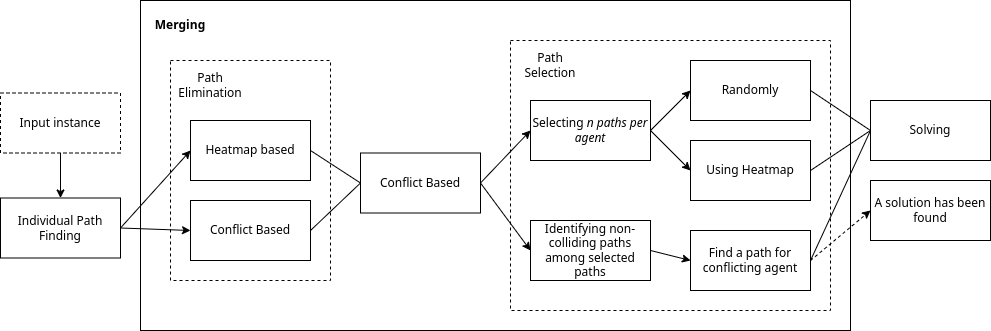
\includegraphics[width=\widthimg]{img/overview_merging_path_selection.drawio.png}
\end{figure}



\subsection{Towards a (partial) plan}

In this section, we explain the method for achieving the first objective outlined above. To summarize, the aim is to identify a partial plan \(\hat{\Pi}\) with the maximum amount of agents.  The corresponding encoding for this approach is provided in Listing~\ref{lst:ps_encoding}.

\begin{minipage}[H]{\linewidth}
\begin{lstlisting}[style=mystyle, caption={Building a conflict free \(\tau'\)}, label={lst:ps_encoding}]
    % Defining collision & possible_path
    possible_path(R,I):- at(R,I,_,_), not path_killed(R,I). |\label{line:possible_path}|
    
    % Constructing a (partial) plan
    {selected_path(R,I) : possible_path(R,I) }1 :-  agent(R). |\label{line:selecting_candidate}|

    collision((R1,P1),(R2,P2),T) :- |\label{line:vertex_collision}|
        R1 != R2, at(R1,P1,V,T), at(R2,P2,V,T),
        selected_path(R1,P1), selected_path(R2,P2).

    collision((R1,P1),(R2,P2),T) :- |\label{line:edge_collision}|
        R1 != R2, at(R1,P1,V1,T), at(R1,P1,V2,T+1), at(R2,P2,V2,T), 
        at(R2,P2,V1,T+1), selected_path(R1,P1), selected_path(R2,P2).
    
    :- collision((R1,P1),(R2,P2),_), |\label{line:no_collision}|
        selected_path(R1,P1), 
        selected_path(R2,P2).

    selected_agent(R) :- selected_path(R,_).  |\label{line:select_agent}|    

    #maximize {1@1,R : selected_path(R,_)}. |\label{line:more_agent}|
\end{lstlisting}
\end{minipage}

Up to this step of Path Selection, paths could have been labeled as either \textbf{selected} or \textbf{killed}. For the remaining paths, line~\ref{line:possible_path} labels them as \(possible\_path/2\). Then, line~\ref{line:selecting_candidate} selects paths from the candidates, ensuring that at most one path per agent is chosen for the output. Following this, lines~\ref{line:vertex_collision} and~\ref{line:edge_collision} define vertex and edge collisions, respectively, among the selected paths. The associated constraint specified in line~\ref{line:no_collision} ensures that the set of \textbf{selected paths} does not contain any collisions. Lastly, the optimization statement in line~\ref{line:more_agent} aims to maximize the number of \textbf{selected paths}, ensuring the selection of as many paths as possible.


\subsection{Towards a subgraph}

The second objective discussed in~\ref{sec:ps} can defined as a pre-processing for a MAPF algorithm. Contrary to the first objective, we require at least one path for each agent. To do so, multiple approaches can be used. By definition, the output of IPF can be used directly. We will, however, describe different approaches to select some paths per agent. 

The approaches that we describe are based on the output of the encoding described in Listing~\ref{lst:ps_encoding}.
The objective is to populate the set of conflict-free paths with paths of agents involved in conflicts. We define two primary approaches:

\noindent\textbf{Utilizing Global Heatmaps:} The first approach involves using GH and similar approaches used in Path Elimination process. This can be done either by employing the Heatmaps computed during the Path Elimination process or by recalculating them using the possible paths issued from~\ref{lst:ps_encoding}  (or from IPF, if all paths have been eliminated)..

\noindent\textbf{Path Conflict Composition:} The second approach relies on path conflict composition, as outlined in Listing~\ref{lst:conflict_based_path_elimination}. Similarly to the heatmap approach, the path conflict composition can be derived either from the Path Elimination process or can be recomputed based on the possible paths obtained through path selection.


We then convert the different paths into the new vertices and edges using the following encoding~\ref{lst:converting_paths_to_subgraph}.

\begin{minipage}[H]{\linewidth}
\begin{lstlisting}[style=mystyle, caption={Converting path to subgraph}, label={lst:converting_paths_to_subgraph}]
    nvertex(V) :- selected_path(R,I), at(R,I,V,_).
    nedge(U,V) :- 
        edge(U,V), 
        nvertex(U), 
        nvertex(V).
\end{lstlisting}
\end{minipage}


\subsection{Evaluating approaches}

We introduced different Path Elimination approaches coupled with Path  Selection, in order to evaluate them, we introduce four metrics. These metrics require a reference to compare Path Selection efficiency. We then introduce a ``brute-force'' Path Selection approach that computes what could be defined as the best output possible for Path Selection\footnote{In our case, the best output possible is a partial plan \(\hat{\Pi}\) as close as possible to a complete valid plan \(\Pi\)}.  This approach is not used in practice because of its huge computation time.


\begin{minipage}[H]{\linewidth}
\begin{lstlisting}[style=mystyle, caption={``Brute-force'' PS approach}, label={lst:brut_force_ps_encoding}]
    % Defining collision & possible_path
    collision((R1,P1),(R2,P2),T) :- 
        R1 != R2, 
        at(R1,P1,V,T), 
        at(R2,P2,V,T).

    collision((R1,P1),(R2,P2),T) :- 
        R1 != R2, 
        at(R1,P1,V1,T), 
        at(R1,P1,V2,T+1), 
        at(R2,P2,V2,T), 
        at(R2,P2,V1,T+1).

    possible_path(R,I):- at(R,I,_,_).

    % Constructing set of non conflicting paths
    {usable_path(R,I) : possible_path(R,I) } :- agent(R).

    :- collision((R1,P1),(R2,P2),_), 
        usable_path(R1,P1), 
        usable_path(R2,P2).

    :- selected_path(R,I), not usable_path(R,I).

    % Constructing a partial plan
    {selected_path(R,I) : possible_path(R,I) }1 :- agent(R).

    :- collision((R1,P1),(R2,P2),_), 
        selected_path(R1,P1), 
        selected_path(R2,P2).

    #maximize {1@1,R : selected_path(R,I)}.
    #maximize {1@2,R,I : usable_path(R,I)}.

\end{lstlisting}
\end{minipage}

The major reason for the long computation time required by the ``brute-force'' PS approach is the identification of vertex and edge conflicts.

We introduce metrics to assess and compare the outcomes of various Path Selection approaches. We will compare the results of approaches to the brut-force output. To do so, we introduce two functions \(brutforce\) and \(approach\) which both take as argument a predicate name and return the associated set of facts. For instance, \(approach(selected\_path/2)\) returns all the selected paths of the approach in a tuple form.

\begin{equ}[H]
    \begin{equation}\label{math:relevance}
        relevance = \frac{|approach(selected\_agent/1) \cap brutforce(selected\_agent/1)|}{|approach(selected\_agent/1) \cup brutforce(selected\_agent/1)|}
    \end{equation}
\caption{Relevance}
\end{equ}

\textbf{Relevance} computes the proportion of common selected agent designated by the approach with brutforce output.

\begin{equ}[H]
    \begin{equation}\label{math:absolute_relevance}
        absolute\_relevance = \frac{|approach(selected\_agent/1)|}{|approach(agent/1)|}
    \end{equation}
\caption{Absolute Relevance}
\end{equ}

\textbf{Absolute Relevance} evaluates the proportion of conflict-free agents found by the approach.


\begin{equ}[H]
    \begin{equation}\label{math:precision}
        precision = \frac{|approach(selected\_path/2) \cap brutforce(usable\_path/2)|}{|approach(selected\_path/2) \cup brutforce(usable\_path/2)|}
    \end{equation}
\caption{Precision}
\end{equ}

\textbf{Precision} evaluate capacity of the approach to select path that are present in the biggest set of conflict-free paths possible. 

\begin{equ}[H]
    \begin{equation}\label{math:chunk_proportion}
        chunk_proportion = \frac{|approach(path\_killed/2)|}{|brutforce(possible\_path/2)|}
    \end{equation}
\caption{Chunk Proportion}
\end{equ}

\textbf{Chunk Proportion} evaluate the proportion of path killed compared to the number of paths. 




\chapter{(Partial) Solving}
In this chapter, we will introduce the two solving approaches that we explored. Solving can be performed using already computed-paths or a subgraph defined by paths.

Solving in both cases is basically performed using the encoding defined in Listing~\ref{lst:solver}.

\begin{minipage}[H]{\linewidth}
\begin{lstlisting}[style=mystyle, caption={Encoding of final solver}, label={lst:solver}, numbers=left, ,escapechar=|]
    time(1..horizon).

    at(R,P,0) :- start(R,P).

    { move(R,U,V,T) : nedge(U,V)} 1 :- agent(R), time(T).

    at(R,V,T) :- move(R,_,V,T).
            :- move(R,U,_,T), not at(R,U,T-1).

    at(R,V,T) :- 
        at(R,V,T-1), 
        not move(R,V,_,T), 
        time(T).

    :- {at(R,V,T)}!=1, agent(R), time(T).|\label{line:one_position_at_a_time}|

    :- { at(R,V,T) : agent(R) }  > 1, nvertex(V), time(T).
    :- move(_,U,V,T), move(_,V,U,T), U < V.

    goal_reached(R) :- at(R,V,horizon), goal(R,V). |\label{line:ipf_goal_reached}|

    #maximize{1,R : goal_reached(R)}. |\label{line:maximize_goal_reached}|
\end{lstlisting}
\end{minipage}


This encoding is derived from the MAPF encoding illustrated in Listing~\ref{lst:base_mapf_encoding} with two significant modifications. The first modification involves the redefinition of movement predicates. Instead of relying on \(vertex/1\) and \(edges/2\), movement is now defined on \(nvertex/1\) and \(nedge/2\), which are generated from the encoding detailed in Listing~\ref{lst:converting_paths_to_subgraph}.

The second distinction is highlighted in lines~\ref{line:ipf_goal_reached} and~\ref{line:maximize_goal_reached}. Unlike classical MAPF, which either provides a complete solution or returns unsatisfiable if no solution exists, the solver in this context can produce a partial solution. This means that due to the steps taken to reduce the complexity MAPF problem, there is a possibility that the solver might not find a complete solution the way we defined it. However, it is possible to extend the algorithm to guarantee the solution by relaxing selected paths -- in the worse case, we relax all selected paths. Which correspond to classical MAPF solving. 


In order to highlight the differences between the two different kinds of solving approaches, we introduce an example in figure~\ref{fig:partial_solving_example}; a \(\tau\) result of IPF of a MAPF problem \(\mathcal{P}\).

\begin{figure}[H]
    \centering
    \caption{Example for solving approaches. Having a \(|\tau| = 3\) as result of IPF}\label{fig:partial_solving_example}
    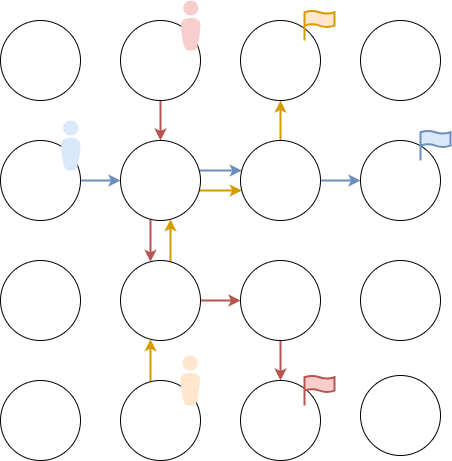
\includegraphics[width=9cm]{img/partial_solving_example.png}
\end{figure}




\section{Pre-computed paths}
As mentioned in the Path Selection section~\ref{sec:pathselection}, the output can vary based on the specified objective. In the context of the primary objective, which aims to construct a (partial) plan, we utilize the set of \textbf{selected paths} to generate \textbf{pre-computed paths}. This translation is achieved through the following rules:

\begin{minipage}[H]{\linewidth}
\begin{lstlisting}[style=mystyle]
    at(R,V,T) :- selected_path(R,I), at(R,I,V,T). |\label{line:selected_to_at}|
\end{lstlisting}
\end{minipage} 
\noindent Through line~\ref{line:selected_to_at}, we ensure that the selected paths are incorporated into the solution. Conversely, for agents without a selected path, the encoding is employed to compute their paths.

\begin{figure}[H]
    \centering
    \caption{Possible output for Path Selection \& Pre computed paths}\label{fig:pre_computed_path_solving}
    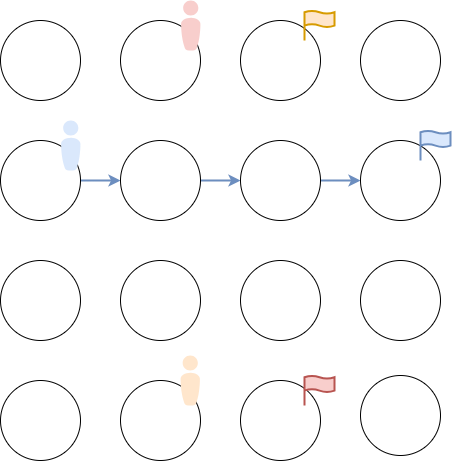
\includegraphics[width=9cm]{img/pre_computed_path_solving.drawio.png}
\end{figure}

Figure~\ref{fig:pre_computed_path_solving} describes a partial plan \(\hat{\Pi}\) where only blue agent has a path. Partial Solving now computes path for the two remaining agents, which is, hopefully easier than computing paths for the all three. In the example outlined in figure~\ref{fig:pre_computed_path_solving}, the solving requires a makespan of five.

\section{Subgraph}

The second objective described in Section~\ref{sec:pathselection} aims to create a subgraph in order to reduce the size of the problem. From the paths in Figure~\ref{fig:partial_solving_example}, we obtain the subgraph shown in Figure~\ref{fig:subgraph_solving}.

\begin{figure}[H]
    \centering
    \caption{Example for solving approaches. Having a \(|\tau| = 3\) as result of IPF}\label{fig:subgraph_solving}
    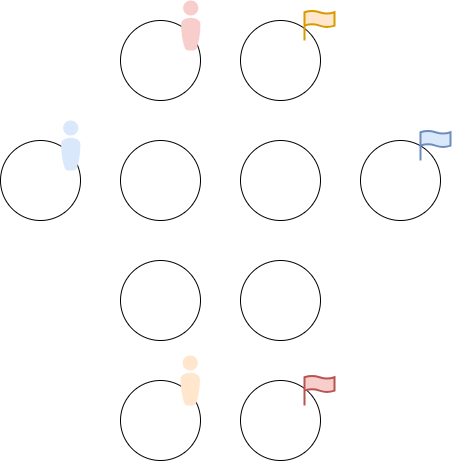
\includegraphics[width=9cm]{img/subgraph_solving.png}
\end{figure}

Contrary to pre-computing path, we aim to reduce the size of the graph the agents can move on. Applying MAPF on the problems described in figure~\ref{fig:subgraph_solving} can find a solution with a makespan of 4.

The two approaches presented can be used as one. 

\subsection{Subgraphs Extension Strategies}

In practice, the subgraph solving approach seems to not be enough to fully solve instances; the agents seem to require too many additional time steps in order to ``solve conflict''. Thus, we introduce two strategies in order to extend subgraphs. 

\subsubsection{Corridor}

The corridor strategy~\cite{surynek2023candidate} is engineered to augment the subgraph-solving process by incorporating neighboring vertices and their associated edges directly into the sub-graph. Corridors can vary in size, allowing for different levels of expansion. Figure~\ref{img:corridor} illustrates a corridor of size one.

\begin{figure}[H]
    \centering
    \caption{Example of corridor}\label{img:corridor}
    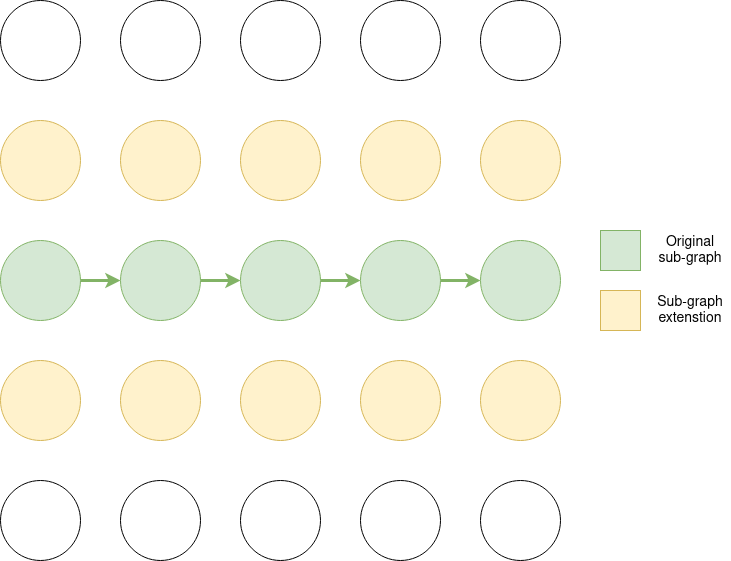
\includegraphics[width=\widthimg]{img/corridor.drawio.png}
\end{figure}

The following encoding in Listing~\ref{lst:corridor_encoding} describe how corridors for paths can be computed.

\begin{minipage}[H]{\linewidth}
\begin{lstlisting}[style=mystyle, caption={Corridor extension encoding}, label={lst:corridor_encoding}]
    #const corridor_level = 2.

    corridor(V,0) :- selected_path_for_corridor(R,I), at(R,I,V,_).
    
    corridor(V,K+1) :- 
        K < corridor_level,
        corridor(U,K),
        edge(U,V).

    nvertex(V) :- corridor(V,_).
\end{lstlisting}
\end{minipage}

Predicate \(selected\_path\_for\_corridor/2\) highlights a path that requires a corridor extension.

With a sufficiently large \(k\), the entire graph can be covered; using a large corridor could essentially revert the problem back to a classical MAPF scenario.

In practice, corridors are created only for paths involved in conflicts, and a choice can be made to create corridors for only one of the two agents involved in a conflict.

\subsubsection{Diamond}

The diamond extension strategy involves expanding the sub-graph by incorporating diamond-shaped arrangements of vertices around conflicting vertices. As illustrated in figure~\ref{img:diamond}, various levels of diamond extension can be applied, each increasing the size of the sub-graph and thereby expanding the possibilities for conflict resolution.

\begin{figure}[H]
  \centering
  \caption{Example of diamond of size 1 and 2}\label{img:diamond}
  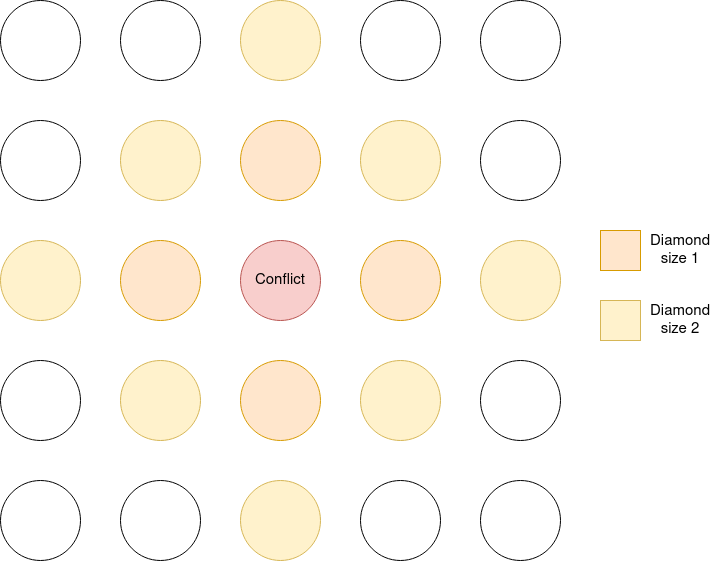
\includegraphics[width=\widthimg]{img/diamond.drawio.png}
\end{figure}


The encoding in Listing~\ref{lst:corridor_encoding} describes how diamonds are computed. As for corridors, the predicate \(selected\_vertex\_for\_diamond/1\) highlight a vertex that requires a diamond extension. In practice, we apply diamond extension on every conflict induced by the set of paths composing the subgraph. 

\begin{minipage}[H]{\linewidth}
\begin{lstlisting}[style=mystyle, caption={Diamond extension encoding}, label={lst:diamond_encoding}]
    #const diamond_level = 2.
    diamond(V,0) :- selected_vertex_for_diamond(V).
    
    diamond(V,S+1) :- 
        diamond(U,S), 
        S<diamond_level, 
        edge(U,V).
    
    nvertex(V) :- diamond(V,_).
\end{lstlisting}
\end{minipage}



\chapter{Benchmarks \& Conclusion}

\section{Benchmarks}

 We evaluate different approaches against the base MAPF encoding introduced in section~\ref{sec:background_mapf}. A witness approach is also evaluated. It consists of one random path per agent converted to a subgraph. Then applying the partial solver~\ref{lst:solver}. It aims to define a referential for the benchmark where shortest path are selected randomly. All used approaches in the benchmark are described in appendix tables~\ref{tbl:approach_ref_and_desc}.

At first, we introduce in Table \ref{tbl:nomenclature_approach} the nomenclature used to name the approaches:

\begin{table}[H]
    \centering
    \caption{Nomenclature of approaches names}
    \label{tbl:nomenclature_approach}
    \begin{tabular}{@{}c|c|c@{}}
    Step Name & Description & Identifier \\ \midrule
    \multirow{2}{*}{IPF} & No Additional path computed & \textbf{N} \\
     & Additional Path computed & \textbf{A} \\ \midrule
    \multirow{2}{*}{Path Elimination} & Simple threshold & \textbf{St} \\
     & Summed Heatmap & \textbf{Sh} \\ \midrule
    \multirow{2}{*}{\begin{tabular}[c]{@{}c@{}}Solving strategy\\ (can be both)\end{tabular}} & Pre-computed path & \textbf{Pc} \\
     & Subgraph & \textbf{Sg} \\ \midrule
    \multirow{2}{*}{Subgraph strategy} & Corridor & \textbf{C} \\
     & Diamond & \textbf{D}
    \end{tabular}
\end{table}

The benchmark were run on a Intel Core i7-4470 @ 3.60ghz with 16GiB of RAM with at most 5 minutes are allowed for each instances. The following values were used for various computations:

\begin{minipage}[H]{\linewidth}
\begin{itemize}
    \item 15 paths requested (30 paths if additional paths are requested)
    \item 1 paths retrieved for the killed agent for the subgraph approach
    \item A bias of 1 for the simple threshold
    \item 70\% of the highest summed heatmap paths are killed
    \item Corridors extension of size one
    \item Diamonds extension of size two  
\end{itemize}
\end{minipage} 


\subsection{Global result}

 Table~\ref{tbl:path_computation_time} shows; the identifier of the approach. The number of instance where it found a (partial) solution and last property outlined shows the average time required to compute a solution with a modified horizon (0 means that the horizon is equal to the makespan). Note that additional horizon is computed for Base MAPF for comparison purpose.


\begin{table}[H]
\begin{center}
\caption{Approaches: focus on average computation time}
\label{tbl:path_computation_time}
\begin{tabular}{@{}lllllll@{}}
\toprule
 \multicolumn{1}{c}{\multirow{2}{*}{Approach}} & \multirow{2}{*}{\# SAT} & \multicolumn{5}{c}{Average time (in sec)} \\ \cmidrule(l){3-7}  
\multicolumn{1}{c}{} &  & \multicolumn{1}{l|}{Horizon} & 0 & 1 & 3 & 5 \\ \midrule
NStPc & 41 & \cellcolor{lightgrey} & 86.3 & 110.8 & 136.7 & 164.3  \\
NStSgC & 44 & \cellcolor{lightgrey} & 14.7 & 29.4 & 38.0 & 47.0  \\
AShSg & 44 & \cellcolor{lightgrey} & 16.7 & 29.9 & 38.9 & 48.0  \\
AStPc & 39 & \cellcolor{lightgrey} & 128.2 & 152.6 & 178.7 & 206.0  \\
MAPF & 44 & \cellcolor{lightgrey} & 25.4 & 34.1 & 52.6 & 72.3  \\
NStSg & 44 & \cellcolor{lightgrey} & 14.5 & 29.1 & 37.8 & 46.6  \\
AStSgCD & 37 & \cellcolor{lightgrey} & 153.7 & 161.2 & 169.4 & 177.8  \\
NShSg & 44 & \cellcolor{lightgrey} & 14.3 & 28.5 & 37.4 & 46.6  \\
NShSgPc & 37 & \cellcolor{lightgrey} & 152.0 & 159.3 & 167.1 & 175.4  \\
AStSgPc & 37 & \cellcolor{lightgrey} & 153.4 & 160.9 & 169.1 & 177.5  \\
AStSg & 43 & \cellcolor{lightgrey} & 30.9 & 39.5 & 48.5 & 58.0  \\
Witness & 44 & \cellcolor{lightgrey} & 9.0 & 17.4 & 26.0 & 34.1  \\
NShSgPcCD & 40 & \cellcolor{lightgrey} & 92.7 & 100.4 & 108.7 & 117.6  \\
NStSgD & 44 & \cellcolor{lightgrey} & 14.6 & 29.5 & 38.1 & 47.1  \\
NShPc & 41 & \cellcolor{lightgrey} & 101.9 & 114.0 & 141.3 & 170.1  \\
NStSgPc & 38 & \cellcolor{lightgrey} & 131.5 & 138.6 & 146.2 & 154.5  \\
AShSgCD & 44 & \cellcolor{lightgrey} & 17.2 & 30.5 & 39.6 & 48.9  \\
NStSgCD & 44 & \cellcolor{lightgrey} & 14.7 & 29.6 & 38.3 & 47.2  \\
\end{tabular}
\end{center}
\end{table}


 Table \ref{tbl:path_computation_time} shows the disparity of efficiency among Plan Merging approaches. Particularly noteworthy is the \textbf{AShSg} approach, which stands out as the fastest among the tested methods. As expected, longer computation time is observed for approaches using additional paths in approaches like \textbf{AStSg}, \textbf{AStSgPc}, and \textbf{AStPc}.
It appears that precomputed paths approaches often times out or, more likely, produces unsat results. This can be attributed to way the paths are forced, described in our methodology, inevitably induces collision. Figure~\ref{fig:precomputed_path_conflict} illustrates a scenario where conflict(s) are inevitable using the pre-computed paths approach.
In all cases, the witness approach seems to be a faster approach while providing for each instances a solution.
\begin{figure}[H]
    \centering
    \caption{Inevitable conflict example for pre-computed path strategy}\label{fig:precomputed_path_conflict}
    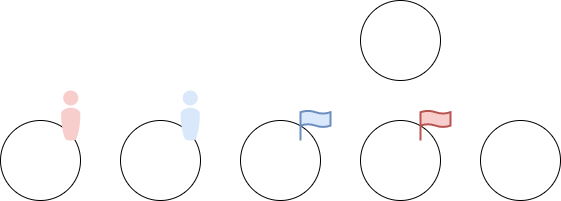
\includegraphics[width=\widthimg]{img/precomputed_path_conflict.drawio.png}
\end{figure}


With table~\ref{tbl:path_proportion}, we focus on the. "\# Fully solved instances" column refers to scenarios where all agents obtain a path. This table also presents the expected proportion of paths found given a modified horizon.

\begin{table}[H]
\begin{center}
\caption{Approaches: focus on solving path proportion}
\label{tbl:path_proportion}
\begin{tabular}{@{}lllllll@{}}
\toprule
 \multicolumn{1}{c}{\multirow{2}{*}{Approach}} & \multirow{2}{*}{\# fully solved} & \multicolumn{5}{c}{Expected \% agent with a path} \\ \cmidrule(l){3-7}  
\multicolumn{1}{c}{} &  & \multicolumn{1}{l|}{Horizon} & 0 & 1 & 3 & 5 \\ \midrule
NStPc & 24 & \cellcolor{lightgrey} & 86 & 87 & 88 & 90  \\
NStSgC & 37 & \cellcolor{lightgrey} & 97 & 97 & 98 & 98  \\
AShSg & 39 & \cellcolor{lightgrey} & 97 & 97 & 98 & 98  \\
AStPc & 22 & \cellcolor{lightgrey} & 80 & 80 & 82 & 83  \\
MAPF & 44 & \cellcolor{lightgrey} & 100 & 100 & 100 & 100  \\
NStSg & 37 & \cellcolor{lightgrey} & 97 & 97 & 98 & 98  \\
AStSgCD & 17 & \cellcolor{lightgrey} & 72 & 72 & 74 & 75  \\
NShSg & 37 & \cellcolor{lightgrey} & 96 & 96 & 97 & 98  \\
NShSgPc & 23 & \cellcolor{lightgrey} & 77 & 78 & 78 & 80  \\
AStSgPc & 17 & \cellcolor{lightgrey} & 72 & 72 & 74 & 75  \\
AStSg & 37 & \cellcolor{lightgrey} & 97 & 97 & 98 & 98  \\
Witness & 38 & \cellcolor{lightgrey} & 96 & 97 & 97 & 98  \\
NShSgPcCD & 21 & \cellcolor{lightgrey} & 83 & 83 & 84 & 85  \\
NStSgD & 37 & \cellcolor{lightgrey} & 97 & 97 & 98 & 98  \\
NShPc & 31 & \cellcolor{lightgrey} & 88 & 89 & 89 & 90  \\
NStSgPc & 15 & \cellcolor{lightgrey} & 75 & 76 & 77 & 78  \\
AShSgCD & 39 & \cellcolor{lightgrey} & 97 & 97 & 98 & 98  \\
NStSgCD & 37 & \cellcolor{lightgrey} & 97 & 97 & 98 & 98  \\
\end{tabular}
\end{center}
\end{table}


This table confirms result concluded with table~\ref{tbl:path_proportion}. Further emphasizing the effectiveness of the \textbf{AShSg} approach, which, among other, have the highest number of fully solved instances.  It also confirms that pre-computed paths approach do not perform well since it register the lowest score in terms of number of fully solved instances and in terms of expected proportion of agent with a path.
The data also indicates that combining Diamond and Corridor extensions does not appear to enhance the solving process. In fact, it even results in worse results compared to similar approaches without these extensions, as evidenced by \textbf{NShSgCD} compared to \textbf{NShSg} and \textbf{AStSgCD} compared to \textbf{AStSg}.
Furthermore, we can notice multiple approaches that are providing really high expected proportion of fully solved instance; \textbf{NStSg}, \textbf{NStSgCD}, \textbf{NStSgD}, \textbf{NStSgC} and \textbf{AStSg}.
Additionally, multiple approaches demonstrate high expected proportions of fully solved instances, including \textbf{NStSg}, \textbf{NStSgCD}, \textbf{NStSgD}, \textbf{NStSgC}, and \textbf{AStSg}.

It is noteworthy that increasing the horizon does not significantly impact the solving proportion. However, as expected, raising the horizon, always improve the ``expected \% agent with a path''.

From these tables, we selected the following approaches; \textbf{MAPF}, \textbf{Witness}, \textbf{AShSg}, \textbf{AStPc}, \textbf{AStSg} and \textbf{NShSg}.

\begin{figure}[H]
    \centering
    \caption{Cactus plot given selected approaches}\label{fig:cactus}
    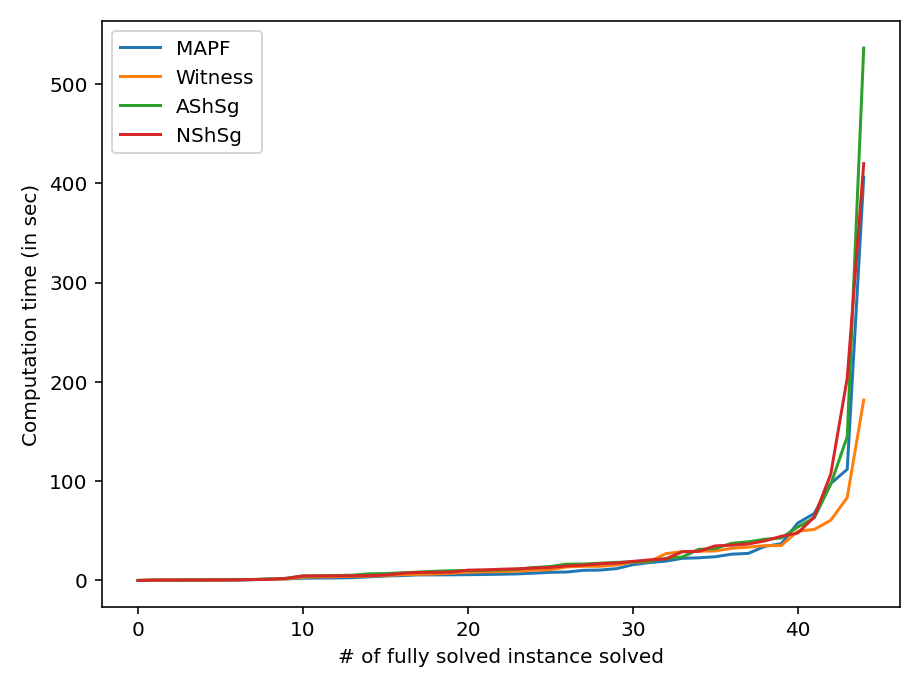
\includegraphics[width=\widthimg]{img/plt_cactus.png}
\end{figure}


The plot illustrated in Figure~\ref{fig:cactus}, shows the performance of some approaches. As computed for table~\ref{sec:pathselection}, to be considered as solved, an approach must find a path for all agents. 

Plan Merging approaches can provide a partial solution faster than the base MAPF encoding, but have worse result if we try to reach a complete solution. Given the great performance of the witness solver, it seems that the Path Selection processes we defined is not efficient. It however shows that separating MAPF in two steps improves the computation time. With a better and smarter IPF, we possibly can provide even better results.


\subsubsection{Detailed performance}

From the best approach \textbf{AShSg} outlined by the previous result, we provide in Table~\ref{tbl:approach_decomposition}, the total time and the proportion of each steps composing the approach.

\begin{table}[]
    \centering
    \caption{Approach Decomposition}\label{tbl:approach_decomposition}
    \begin{tabular}{@{}llllll@{}}
    \toprule
    \multicolumn{1}{l|}{\multirow{2}{*}{Step Name}} & \multicolumn{3}{c|}{Total time} & \multicolumn{2}{c}{\% of the process} \\ \cmidrule(l){2-6}  
    \multicolumn{1}{l|}{} & \multicolumn{1}{l|}{Id.} & \multicolumn{1}{c}{AShSg} & \multicolumn{1}{c|}{Witness} & \multicolumn{1}{c}{AShSg} & Witness \\ \midrule
    IPF & \cellcolor{lightgrey} & 49 & 41  &7\% &10\%  \\
    Heatmaps Computation & \cellcolor{lightgrey} & 14 &  - &2\% & - \\
    Summed Heatmap per Path & \cellcolor{lightgrey} & 0 &  - &0\% & - \\
    Path Elimination & \cellcolor{lightgrey} & 7 &  - &1\% & - \\
    Path Selection & \cellcolor{lightgrey} & 8 & 1  &1\% &0\%  \\
    Partial Solving & \cellcolor{lightgrey} & 551 & 352  &87\% &89\%  \\
    \end{tabular}
    \end{table}

    
The table illustrates the time distribution across different steps of the approach. While generating initial paths is relatively efficient, the process of finding partial solutions is a significant portion of the computation time. These insights tells us that  \textbf{partial solving} requires the most an optimization. However, this step depends on all previous steps and on the solver itself. Another possible optimization track is the IPF step which could be improved with a faster programming language. On the other hand the \textbf{witness} approach shows us that one random path is enough to have really good result. 




\section{Conclusion}


\newpage


\section*{References}
\printbibliography[heading=none]

\section*{Appendix}

\begin{table}[H]
    \begin{center}
    \caption{Table of the approaches reference name and their description}
    \label{tbl:approach_ref_and_desc}
    \begin{tabular}{ | p{2cm} | p{8cm}|  } 
        \hline
        Name & Value \\
        \hline
        \hline
        \textbf{NStPc} & No additional path, heatmap simple threshold elimination, pre-computed path on full graph \\
        \hline
        \textbf{NStSg} & No additional path, heatmap simple threshold elimination, subgraph approach \\
        \hline
        \textbf{NStSgPc} & no additional paths, simple threshold elimination, precomputed path on subgraph \\
        \hline
        \textbf{AStPc} & Additional path, heatmap simple threshold elimination, pre-computed path on full graph \\
        \hline
        \textbf{AStSg} & Additional path, heatmap simple threshold elimination, subgraph approach \\
        \hline
        \textbf{AStSgPc} & Additional paths, simple threshold elimination, precomputed path on subgraph \\
        \hline
        \textbf{NStSgC} & No Additional path, heatmap simple threshold elimination, subgraph approach with corridor \\
        \hline
        \textbf{NStSgD} & No Additional path, heatmap simple threshold elimination, subgraph approach with diamond \\
        \hline
        \textbf{NStSgCD} &  No Additional path, heatmap simple threshold elimination, subgraph approach with diamond and corridor \\
        \hline
        \textbf{AStSgCD} &  No Additional path, heatmap simple threshold elimination, subgraph approach with diamond and corridor \\
        \hline
        \textbf{NShPc} & No additional path, summed heatmap elimination, pre-computed path on full graph \\
        \hline
        \textbf{NShSg} & No additional path, summed heatmap elimination, subgraph approach \\
        \hline
        \textbf{NShSgPc} & No additional paths, summed heatmap elimination, precomputed path on subgraph \\
        \hline
        \textbf{AShPc} & Additional path, summed heatmap elimination, subgraph approach \\
        \hline
        \textbf{NShPcCD} & Additional path, summed heatmap elimination, subgraph approach with diamond and corridor \\
        \hline
        \textbf{MAPF} & Classical MAPF approach \\
        \hline
    \end{tabular}
    \end{center}
    \end{table}
\end{document}
